\documentclass{template}
\usepackage{graphicx,parskip,bibunits,appendix,float}
\usepackage[ruled] {algorithm2e}
\usepackage{url,amsmath,amssymb,fancybox,listings,pdfpages,caption,multicol,datetime,rotating, booktabs}
%\usepackage[usenames,dvipsnames]{color}
\usepackage{tgheros}
\usepackage[pagebackref=false,pdffitwindow=true]{hyperref}
\usepackage{natbib}
\usepackage{xcolor,colortbl}
\renewcommand{\arraystretch}{1.5}
\graphicspath{ {images/} }
%NOTE: The hyperref usepackage should be the last \usepackage!!
%NOTE: When pagebackref=true an error will appear at the end of compiling. press `q' to ignore
%NOTE: Referencing Algorithms does not work if this usepackage is before the hyperref include.!!
%NOTE: This is a comment, ignored when the document is compiled
%NOTE: The following document configuration settings generally do not need to be modified
%NOTE: More packages may need to be added to provide additional functionality

\hypersetup{
    pdftitle    = {Report Title},
    pdfauthor   = {Author Name},
    pdfsubject  = {Subject Area},
    pdfkeywords = {Comma separated list of keywords},
    colorlinks  = true, anchorcolor = colIdentifier, filecolor = colIdentifier, urlcolor = colIdentifier,
    linkcolor   = colIdentifier,    %NOTE: change (blue) to (colIdentifier) to have links within the document in Black
    citecolor   = colIdentifier,    %NOTE: change (blue) to (colIdentifier) to have citation links within the document in Black
}

\definecolor{colBackGrnd}{rgb}{1,1,0.8}
\definecolor{colKeys}{rgb}{0,0,1}
\definecolor{colIdentifier}{rgb}{0,0,0}
\definecolor{colComments}{rgb}{0,.5,0}
\definecolor{colString}{rgb}{0,0,1}
\definecolor{colWhite}{rgb}{1,1,1}
\definecolor{LightCyan}{rgb}{0.88,1,1}

\newcommand{\MyHookSign}{\hbox{\ensuremath\hookleftarrow}}

\newtheorem{Theorem}{Theorem}
\newtheorem{Proposition}[Theorem]{Proposition}
\newtheorem{Lemma}[Theorem]{Lemma}
\newtheorem{Proof}[Theorem]{Proof}
\newtheorem{Remark}[Theorem]{Remark}
\newtheorem{Claim}[Theorem]{Claim}
\newtheorem{Example}[Theorem]{Example}
\newtheorem{Definition}[Theorem]{Definition}

%NOTE: Setup for including program listings
\lstset{%
    float=H,
    basicstyle=\ttfamily\footnotesize,
    identifierstyle=\color{colIdentifier},
    keywordstyle=\color{colIdentifier}, %
    stringstyle=\color{colIdentifier},
    commentstyle=\color{colIdentifier}, %
    columns=flexible,
    tabsize=2,
    frame=single,
    extendedchars=true, %
    showspaces=false,
    showstringspaces=false,
    numbers=left, %
    numberstyle=\footnotesize,
    breaklines=true,
    prebreak={\space\MyHookSign},
    language=Java,
    backgroundcolor=\color{colBackGrnd},
    breakautoindent=true, %
    captionpos=b%
} %\hypersetup{colorlinks=true, citecolor=\color{colIdentifier}}

\sloppy %NOTE: To ensure the Right Hand Margin is used (Especially for long URLS)
%NOTE: END of the document configuration settings

\begin{document}
{
\fontfamily{qhv}\selectfont


\DeclareGraphicsExtensions{.jpg,.png,.gif,.pdf}
%NOTE: When inserting Figures if the extension of the graphic file is not provided LaTeX will automatically search
% for the extensions declared above, in the order declared.

\title{\huge{Machine Learning for better healthcare practices}}
\author{Annabelle Macleod}
\degreetitle{BSc(Hons) in Computing Science: Honours Thesis} % Replace with appropriate degree
\rpttype{BSc(Hons}    % Replace MSc with BSc for Honours Degree Year projects.
\principaladviser{Dr. Eyad Elyan}

\beforeabstract
\prefacesection{Abstract}

The healthcare sector is the fastest growing sector in terms of data generation and there has been an increasing interest in recent years in applying the tools of machine learning to the healthcare industry with a view to deliver better and more efficient patient care.\newline
One of the challenges of applying machine learning models to healthcare datasets is that those datasets are frequently severely imbalanced and this can negatively affect the performance of an algorithm.\newline
This project evaluates some of the available techniques to address the issue of class imbalance at data-level:
\begin{itemize}
    \item random under-sampling of the majority class,
    \item  synthetic minority over-sampling technique (SMOTE).
\end{itemize}

After assessing the performance of Random Forest on several health-related datasets, random under-sampling and SMOTE were applied separately to the datasets and the performance of Random Forest was assessed again.
The results obtained show that, while no single technique proved to consistently improve Random Forest performance across all datasets, for some datasets, under-sampling proved to be more successful at improving F1 score, \textit{i.e} suggesting an increase in both sensitivity and precision than SMOTE. However, SMOTE resulted in sensitivity increasing in a statistically significant manner across all dataset when compared to the baseline. The other metrics were not found statistically significantly different.\newline
Given the healthcare context of the data, it was decided that the metric Sensitivity (a high Sensitivity value suggests a low number of false negatives) would be rated as more important than Precision (a low Precision value suggests a high number of false positives) when evaluating algorithm performance.\newline
The results from this project also suggests that there is a strong data-dependent effect on the performance of the algorithm and as such it is not possible to recommend one technique over the other as an absolute, rather both should be investigated with different parameters when studying a new dataset and devising a new machine learning model.\newline




\prefacesection{Acknowledgements}

I would like to thank everyone who has taken an interest in this project and offered advice or suggestions, big or small. 

I would particularly like to thank Dr Eyad Elyan for his guidance, supervision and support during this past year and for encouraging me to submit my own proposal early on.
I would also like to thank Rob, my husband for his continued encouragements, support and patience over the last five years.


\afterpreface \afterabstract

\listofalgorithms   %NOTE: Will generate a list of Algorithms in the Table of Contents Section
\lstlistoflistings  %NOTE: Will generate a list of Program Listings in the Table of Contents Section

%NOTE: Include the relative reference for each chapter to be included
% dividing the thesis file structure into a number of directories aids development
% format: directoryName/filename (the .tex extension is not required for the filename)

\chapter{Introduction}
\pagenumbering{arabic} \setcounter{page}{1}

A large amount of data is produced in the healthcare sector \cite{EMC:2014ve} and much of it remains under utilised and/or under analysed due to either lack of resources (need ref here) or mistrust from patients towards Big Data project \cite{Goldacre:tf}\cite{bcs:2017tl}. About 10\% of the UK's population health data is currently available for research through the clinical practice datalink (GRPD) and represents untapped research resource \cite{Kousoulis:2015ti}. However there have already been some successful development of algorithms to help predict healthcare conditions \cite{Bellon:2013um} and through the analysis of social media streams to spot warning signs of major epidemics \cite{Kostkova:2016ur}.
As such this project aims to use one dataset (or multiple related ones that can be interlinked for better exploration of the data) and analyse the features from the data in order to develop a model that could be used to assist the healthcare profession in cost, trends or diagnosis predictions.


\section{Background}
The healthcare sector is currently one of the fastest growing area of data generation \cite{EMC:2014ve}. Using this data to create a more efficient care delivery system and provide better care to a growing patient base is one of the objective of the IT industry in healthcare. Analysis of large datasets to drive better health outcomes is not new but was traditionally done through large randomised controlled trials (RCT) or systematic reviews \cite{Callahan:2017bz}. Those two types of data collection and analysis are the mainstays of evidence based medicine but present shortcomings in that they pose a challenge in administering such large trials and they typically only gather datas from certain types of patient due to the very restricted inclusion criteria that are usually applied to these studies.
The collection of sample data from the population at large through electronic health record (EHR) can provide large amounts of data across varied patient populations over extensive period of times that would exceed those typically done in RCT (some cohort studies do follow populations over long periods of time but they can present issues with volunteers dropping out of the studies). The gathering of data through continuous health monitoring and from healthcare providers for research purposes would also allow the study of outcomes for patients on multiple medications or suffering from multiple illnesses. If carried out country-wide or even at international level, there would be a high enough amount of patient data to provide robust insights into complex interactions that cannot be revealed through traditional RTC or systematic reviews which tends to focus on narrower criteria of patients.
As early as the 1970s, the use of informatics in healthcare has been evident but the increased production of data, digitisation of patient data as well as as technological advances which allow for real-time monitoring, better at home data collection through the use of wearables and medically developed apps, and large datasets processing has driven the use of  data analytics and machine learning for the healthcare sector \cite{EMC:2014ve}. 
In recent years there have been many publications showing the use of the machine learning to develop better healthcare models, from predicting risk of peripheral artery disease \cite{Ross:2016kh} to predicting emergency department admissions \cite{Peck:2012eg}.
It should however be noted that machine learning is not a magic bullet: not all predicted results will be actionable. For instance there may not be an existing cure for a diagnosis that has been predicted or a model may predict a treatment to be ineffective in certain cases with no existing alternative, which pose ethical concerns as to the action to be taken, this choice should then be considered between patient and physician and falls outwith the remit of what machine learning can do for us \cite{Callahan:2017bz}.

\section{Motivation}
The healthcare sector currently produces large amounts of data every year and this is set to grow.  According to a report from DellEMC, there were already 153 exabytes of healthcare-related data, with a forecast growth of reaching 2,314 exabytes by 2020 \cite{EMC:2014ve}. The same report highlights that healthcare is the fastest growing sector for data production (annual growth of 48\% compared to an average of 40\% across all sectors).  Health related connected devices (e.g. smart hospital beds , drug delivery system) will increase the data produced in the healthcare sector, with predictions suggesting these devices will contribute up to 16\% of the healthcare data by 2020.
Further the increased use of wearables produces even larger amount of personalised health data that are largely unexploited (currently only the manufacturers of the devices or developers of the app used on the device have access to this data unless the users have expressively permitted their use for research (e.g. Apple Heart Study with Stanford University \cite{Anonymous:I2FTN6O4, Medicine:2017wa}). 
However not all of this data is considered useful and one of the challenges to come will be to identify useful data at the right time \cite{EMC:2014ve}.
It is thought that healthcare services will be under increased demands from an ageing populations with chronic conditions, adding pressure to a system where staff shortage can already be an issue \cite{Medicine:2017wa}.
These factors will require healthcare providers worldwide to be more efficient in delivering patient care. Thus developing algorithms that can accurately predicts patients needs based on their devices output or algorithms that can forecast regional trends of illness or healthcare requirements ahead of time would greatly help organisations provide better care for their patients.

\section{Aims and Objectives}
In this project the practice level prescribing dataset from NHS digital for England will be used for all the available years (accessible here https://digital.nhs.uk/data-and-information/publications/statistical/practice-level-prescribing-data). 
This dataset describes prescribing from GP practices in England for years 2012-2018 and is a list of all medicines, dressings and appliances that are prescribed by all practices in England and dispensed in the community each month. This data has been published every month since July 2016. 
\begin{enumerate}
    \item A comprehensive review of the relevant literature will be undertaken to give this project context and explore what work has already been done in this area of research.
    
    \item The data will be preprocessed so as to eliminate any redundant or non useful information and to fit the data to a format better suited to our analysis.
    
    \item The data available will be explored to identify trends in prescribing and various analyses will be carried out to determine which factors may be affecting prescribing by GPs. In order to help with the identification of factors that drive particular prescribing needs, other datasets available from NHS digital may be used such as the supporting information datasets:
        \begin{itemize}
            \item{\% population aged under 18 (https://data.england.nhs.uk/dataset/phe-indicator-92309)}
            \item{\% population aged under 75 mortality rate from various causes}
            \item {population coverage vaccine data}
            \item other indicators available 
        \end{itemize}

    The prescribing data used for this project will only be considered up to and including 2015 as most of the supplementary data for health indicators available publicly only cover years up to 2015.
    
    \item The data will be split into training and testing set so that once a model has been developed, it can be tested against the available data and its accuracy can be determined.
    
    \item The main aim of this project is to develop a model which will allow the forecasting of prescribing needs throughout a year for an average GP practice. In order to develop this model, various factors will be examined for their impact on drug prescription (e.g. time of year, location, vaccine uptake, location, etc). It is hoped that developing such a model would help a GP practice structure their needs for the year e.g. increased need for a type of prescription at certain time of years could lead to review of the causes for this need as well as sending relevant advice to patient or setting up clinic-style appointment for this particular need in order to be more efficient. This could also be useful for pharmacies to adjust their ordering and stock so that required medications are always at hand when needed while less needed medications do not go unused.
    The analysis of the prescribing data could also yield insight into variations on health need based on geographical location, these results together with census data or other available demographic data could inform NHS provisions in certain areas.
    
    \item Finally the model will be tested on the testing data set to establish its accuracy and fit to the available data. These findings will be discussed and compared to other work in the literature.
\end{enumerate}
\section{Key Techniques}
The main language used to analyse the data and develop the model will be R.
The data will be preprocessed to generate usable datasets for the analysis and will be analysed through appropriate statistical methods with the help of various R packages and libraries.
Visualisation techniques using R will be applied to present the data and a model using stepwise logistic regression or random forest algorithm will be used. 
Various contributing factors will be tested for their effect on the models and how those factors impact the accuracy of the models. These models will be tested on a subset of the existing data to determine their accuracy and fit to the test data. 
R studio will be used as a platform for the analysis.

Note: the techniques outlined here may be subjected to change as the project progresses and depending on the size of the data, other platforms (e.g. Hadoop) may eventually be used.

\section{Legal, Social and Ethical Issues}
The use of people healthcare data carries significant legal, social and ethical issues as this type of data is highly personal and confidential. 
All data gathered in the UK falls under the Data Protection Act (1998) and the General Data Protection Rule (GDPR, 2018). This means that data gathered in any context can only be used for the purpose that an individual has expressively agreed to. Therefore patient data can only be used for research purpose and publicly shared if patients have consented to do so. 
The data used for this project was collected from GP practices in England and is a list of all prescribed medication, dressing and appliances prescribed each month. However it does not list who these items where described to, or by which GP. The only data available is the item prescribed along with a practice code and a quantity of the item prescribed. The data is released every month and is already publicly available. This dataset has therefore been approved for release and has been anonymised and consent, where appropriate as already been granted for use of the data for research purpose.
There are no patient level data available in this dataset.
This project aims to develop a model that will allow forecasting of prescribing in GP practices. This can potentially carry some ethical and social issues:
\begin{itemize}
    \item If the model developed was to be used in a real life situation, any inaccuracy in predicted prescribing needs could engender delay in patients accessing their medications or overstocking of medicines that will go unused.
    \item The analysis of the data may reveal some variations between geographical areas and this may have some social implications if those variations are then addressed. For example if an area is found to have low dispensation of vaccines, it may be appropriate for the relevant practices to do a campaign to better promote vaccine uptake as well as to explore the reasons behind this. Such interventions have financial and social cost and need to be planned appropriately to be efficient.
    \item Finally, it is worth considering the end use of such results, for example life or critical illness insurance companies could apply an extra premium based on post code if certain types of prescriptions for chronic illnesses where found to be higher in particular area so it is worth stressing that the end use for the models develop here would not be suited to that effect.
\end{itemize}

\section{Project Plan}
Firstly a healthcare-related dataset will be chosen to carry out the analysis and develop a model. Once the dataset has been selected the data will be preprocessed so as to eliminate any unnecessary columns, or aggregate some tables where appropriate with a view to make the dataset smaller.
The dataset will then be split into training and testing sets. The training set will be used to develop the model, while the testing set will be used to test the fit and accuracy of the model.
In order to develop a suitable model, the existing training data will be presented and explored to identify various trends and those factors that influence them.
Finally a model will be formed and an algorithm will be built.
The model will then be testing with the testing set to determine its fit and accuracy.


\section{Chapter List}
Provide a list of all the chapters within the thesis and a brief summary of the content.

\textbf{Chapter 1 \ref{ch:introduction}} Introduction. 

\textbf{Chapter \ref{ch:Background}} Background Research. 
%This chapter deals with $\ldots$.

\textbf{Chapter \ref{ch:Design}} Design. 
%This chapter deals with $\ldots$.

\textbf{Chapter \ref{ch:Implementation}} Implementation. 
%This chapter deals with $\ldots$.

\textbf{Chapter \ref{ch:Evaluation}} Evaluation \& Testing. 
%This chapter deals with $\ldots$.

\textbf{Chapter \ref{ch:Conclusion}} Conclusion. 
%The conclusions of the thesis are presented.


\section{Conclusion}
This chapter has outlined the main aspects and phases of this project and detailed the motivations for carrying out the research. 
The next chapter will be exploring the current and recent research in the field of healthcare-related data anslytics and machine learning.

\chapter{Literature Review}\label{ch:Background}

This chapter provides some background research on the project and examines some work carried out in the area of research. Firstly, the chapter will give an overview of Machine Learning in general, then supervised machine learning will be discussed in greater details. The chapter will then focus on the use of Machine Learning in the Healthcare sector and the work currently being done in this area. Finally the challenges that arise with the use of machine learning with healthcare related datasets will then be explored. This review does not claim to be exhaustive or systematic and instead focuses on work achieved in recent years, while trying to compare several examples of work that has been done in the field and discuss their reach and limitations.

\section{Machine Learning}
Machine learning is considered to be a branch of artificial intelligence and has been around for decades. It has been defined by Arthur Samuel as ''the programming of a digital computer to behave in a way which, if done by human being or animals would be described as involving the process of learning'' \citep{Samuel:1959vp}.  Technological advances since then have meant that considerable amount of data have been produced and will need to be analyzed. A report by the EMC corporation estimates that newly generated data will grow 40\% a year and that by 2020, the size of the ''digital universe'' will reach 44 zettabytes \citep{EMC:ylTs53OV}. Despite the larger quantity of data being produced daily, as of 2013, only 22\% of the data generated worldwide was considered useful if it were tagged, and less than 5\% was actually analyzed. It is estimated, however that proportion of the data considered useful is likely to reach 35\% by 2020, mostly due to the growth of data from embedded systems \citep{EMC:ylTs53OV}. 
This growth in data production and the advances in computing generally means that the field of machine learning and artificial intelligence have also seen growth and are expected to continue growing \citep{Colombus:wm}. Recent decades have seen sharp increases in computing speed, in turn allowing systems to collect and process large quantities of data very rapidly \citep{Denning:2016fz} . At the same time as computing power increased, the cost of both transistors and storage have decreased markedly: from \$222 per million transistors in 1992 to \$0.06 per million transistors in 2012 and from \$569 per gigabyte of storage in 1992 to \$0.03 per gigabyte in 2012 \citep{Hagel:2013ur}. These two factors combined with increased availability of competent graduates in the field of AI as well as cultural acceptance from the public have allowed the field of machine learning to expand \citep{Evans:sHGdqFvY}. Indeed in 2017, Deloitte predicted that 300 millions smart phones would have on-board neural network machine learning capabilities, meaning that pattern recognition could happen in some instances (e.g. language translation, navigation) without network connectivity \citep{Deloitte:2017wo}.

Although machine learning represents a number of algorithms, it can be broadly categorized in two types: supervised and unsupervised learning (see figure 2.1). In supervised learning, the learning agent will observe some example input-output pairs and learns a function that maps from input to output \citep{Russell:2016tz}. In other words, the goal of supervised learning is to learn a function that can best approximate the relationship between input and output observable in the data \citep{Mullainathan:uy}. 
In contrast, in unsupervised learning, the tasks are generally clustering, representation learning or density estimation(see figure 2.1), i.e. learning the inherent structure of the data without explicitly-provided labels. The lack of labels means that there is no specific way to measure model performance in unsupervised learning \citep{Soni:tr}.

\begin{figure}[H]
\centering
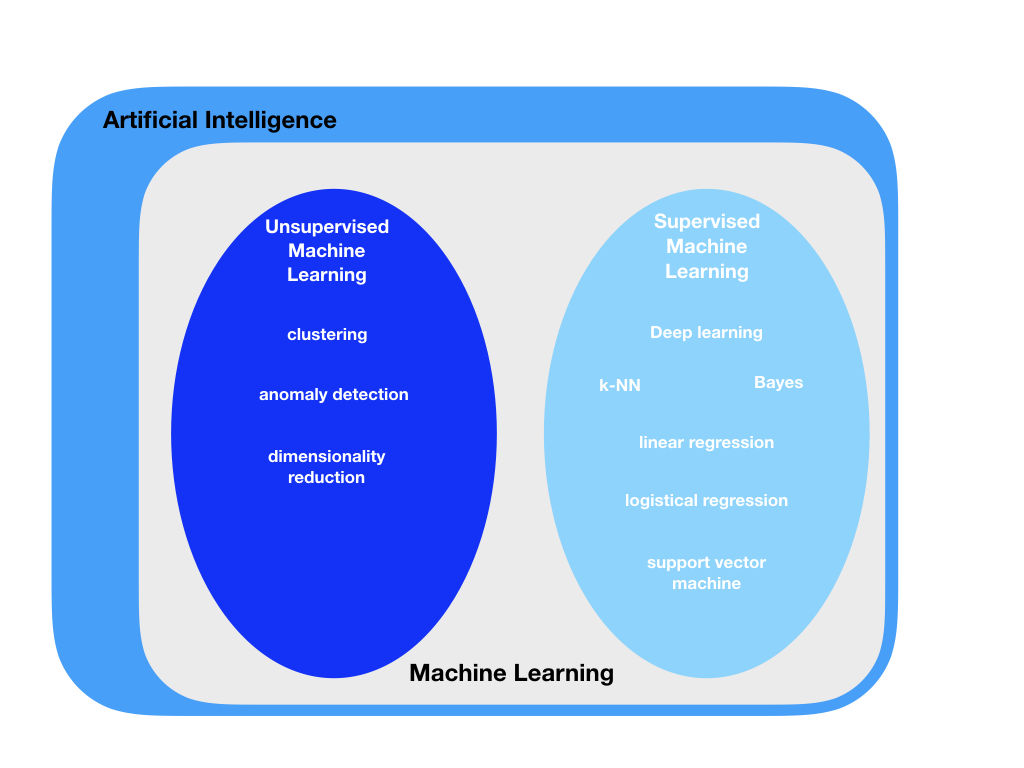
\includegraphics[width=0.8\textwidth]{ThesisTemplate/usingLatex/images/Figure1.png}
\caption{Types of machine learning: this diagram shows examples of algorithms for machine learning and which category they belong to.}
\end{figure}


Machine learning is used in many different sectors from finance to healthcare, through to education and customer relations. Many machine learning algorithms are now used to assist decision making in many fields (e.g. credit scoring \citep{Guegan:2018ey}, medical diagnostic) with many have shown very high performance (Figure 2.2. shows investment in AI (which comprises machine learning) generally by sector).

\begin{figure}[H]
\centering
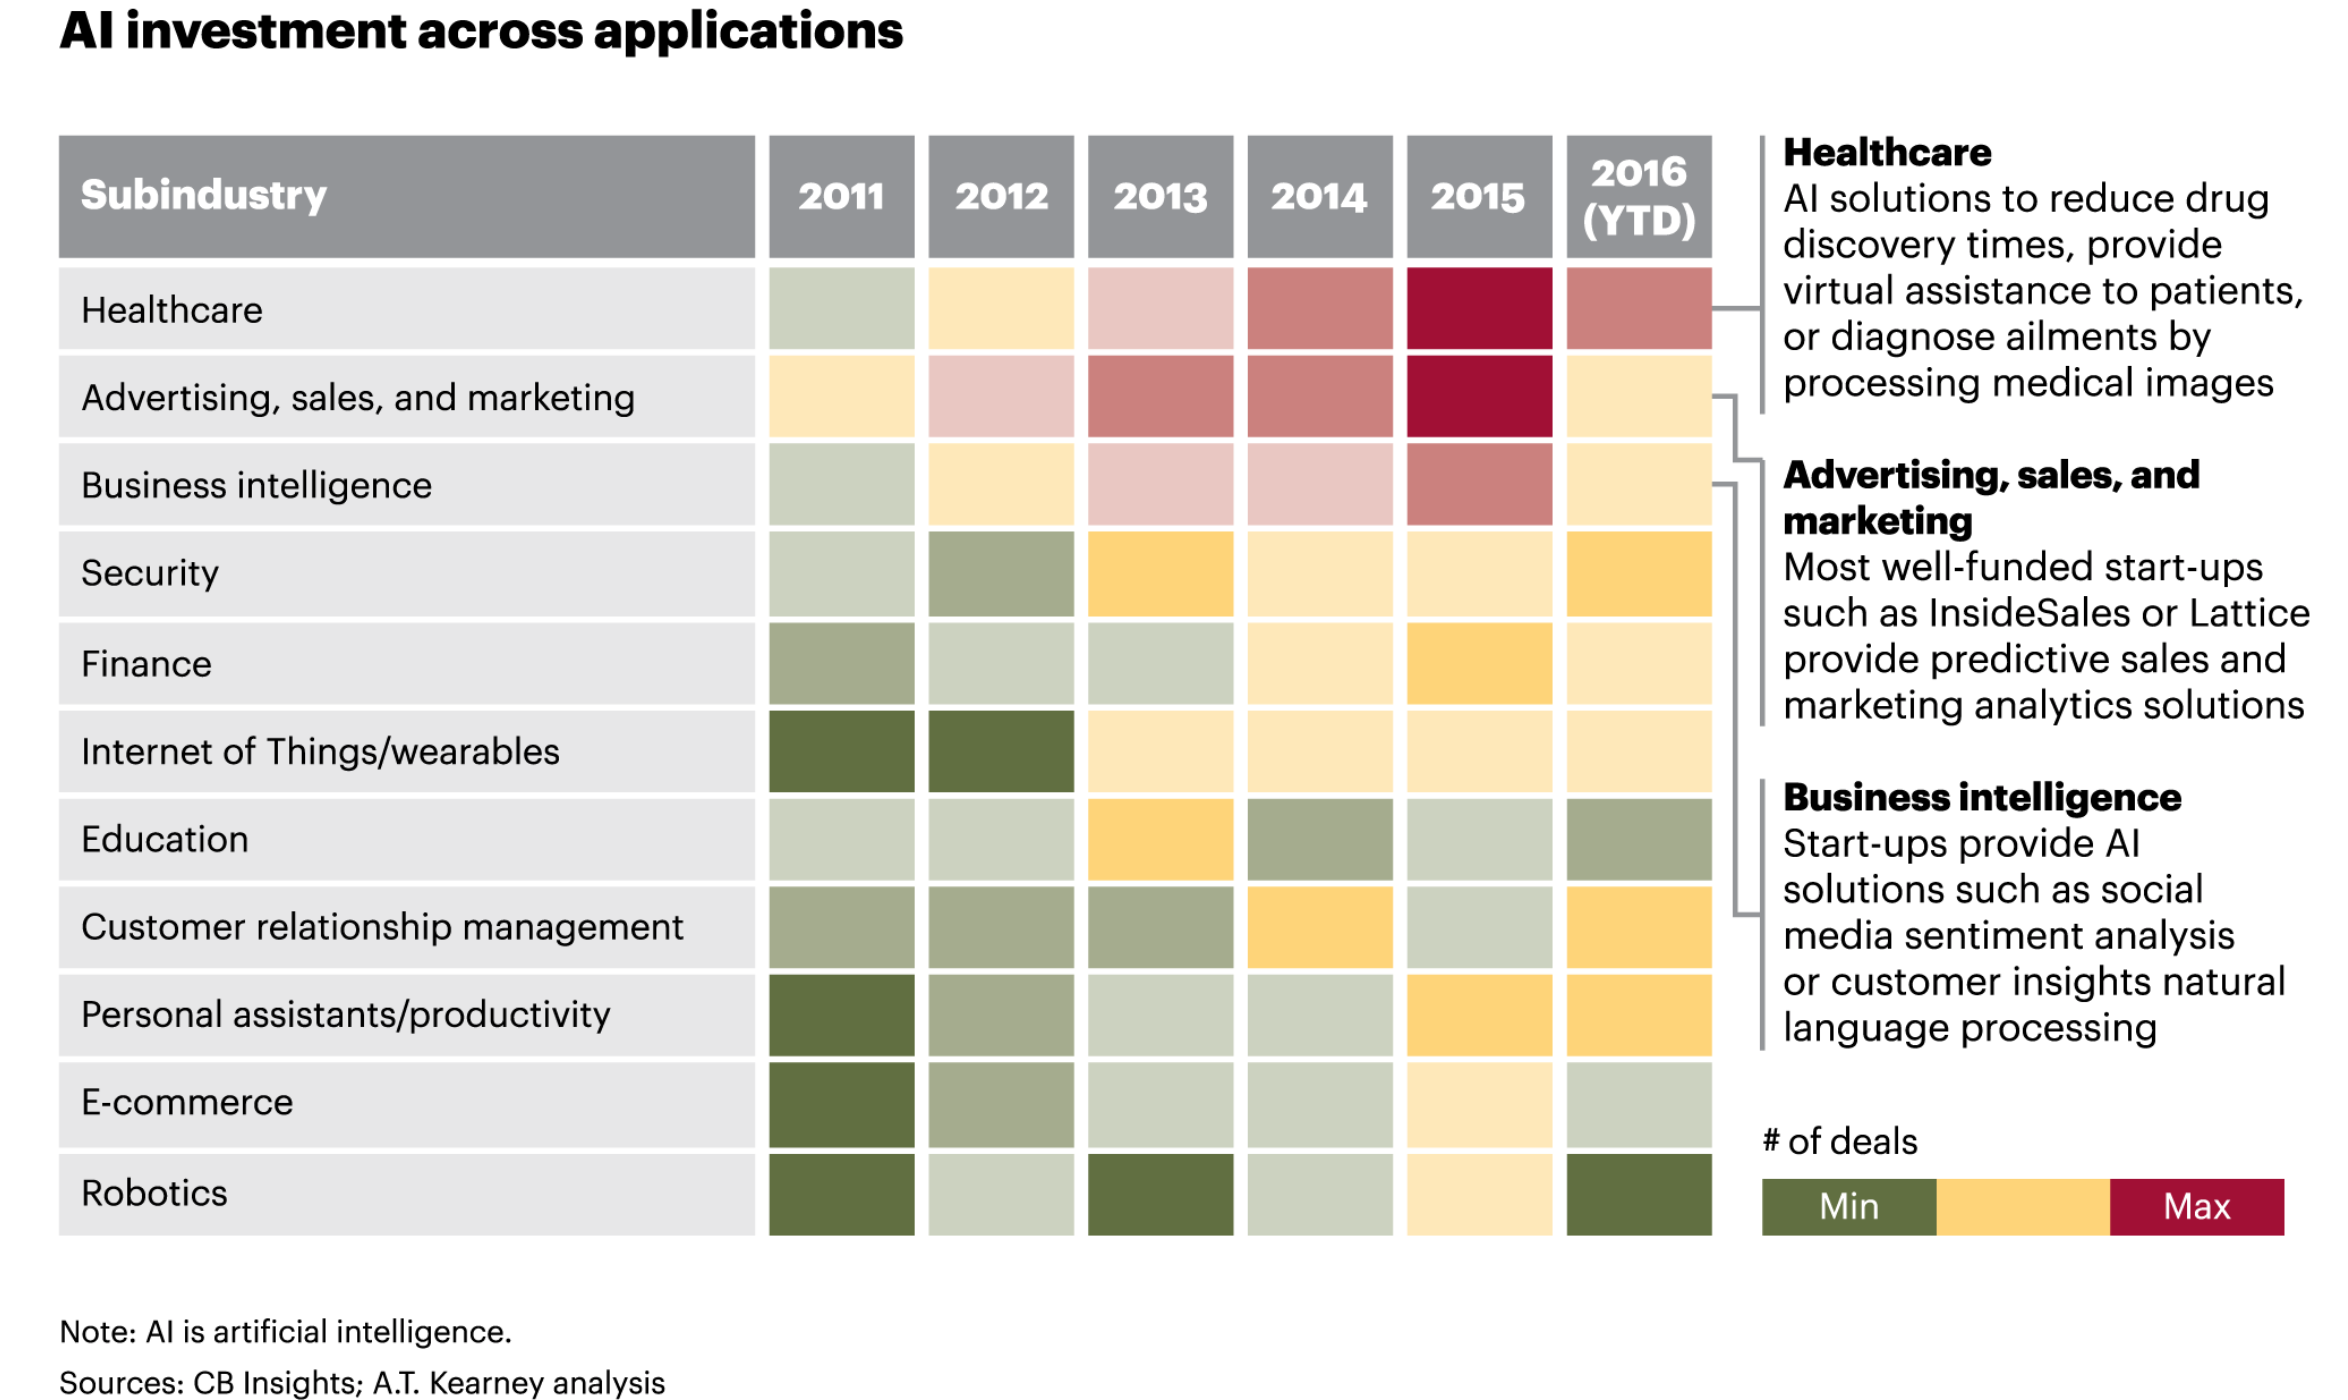
\includegraphics[width=0.8\textwidth]{ThesisTemplate/usingLatex/images/fig2_2.png}
\caption{Investment in AI by sector (source: Will you embrace AI fast enough? \citep{Evans:sHGdqFvY}}
\end{figure}

It is important however to point out that each algorithm will have a True Positive (TP) rate, a False Positive (FP) rate, a True Negative (TN) rate and a False Negative (FN) rate \citep{Ting:2016ue}:
\begin{itemize}
    \item The TP rate is the proportion of correctly identified instances for positive condition of the target label. For example in the case of a given medical diagnostic, TP would be the number of correctly identified sick patients for a given condition.
    \item  FP is the proportion of incorrectly labelled instances for the positive condition of the target label, i.e the number of actually negative instances that have been labelled as positive by the algorithms. 
    \item TN is the proportion of correctly labelled instances for the negative condition of the target label, i.e. how many healthy patients have been appropriately labelled as healthy.
    \item FN is the proportion of incorrectly labelled instances for the negative condition of the target label, i.e. how many sick patients were labelled as healthy by the algorithm.
\end{itemize}

These figures are used to estimate the performance of a given algorithm (more in section 2.2.2) and these parameters must be known when real life decisions are being made. In the cases of very high performing algorithms, there is an increased chance of false positives, which could have unintended real-life consequences (for example in the field of medicine, if a diagnostic of serious illness is made by the algorithm but the patient is healthy, they may have to undergo unnecessary tests to confirm the diagnostic). Equally, a less performing algorithm will a higher rate of false negatives which could also have dire consequences. There are obviously ethical and moral considerations to be taken into account when machine learning algorithms are developed for decision making with real life implications. 

\section{Supervised Machine Learning}
\subsection{Definition}
Supervised learning is typically carried out in the context of classification (mapping input to output labels) or regression problems (mapping input to continuous output). In both cases, the aim is to establish a specific relationship in the input data that will allow the output data to be correctly labelled \citep{Soni:tr}. 

\begin{figure}[H]
    \centering
    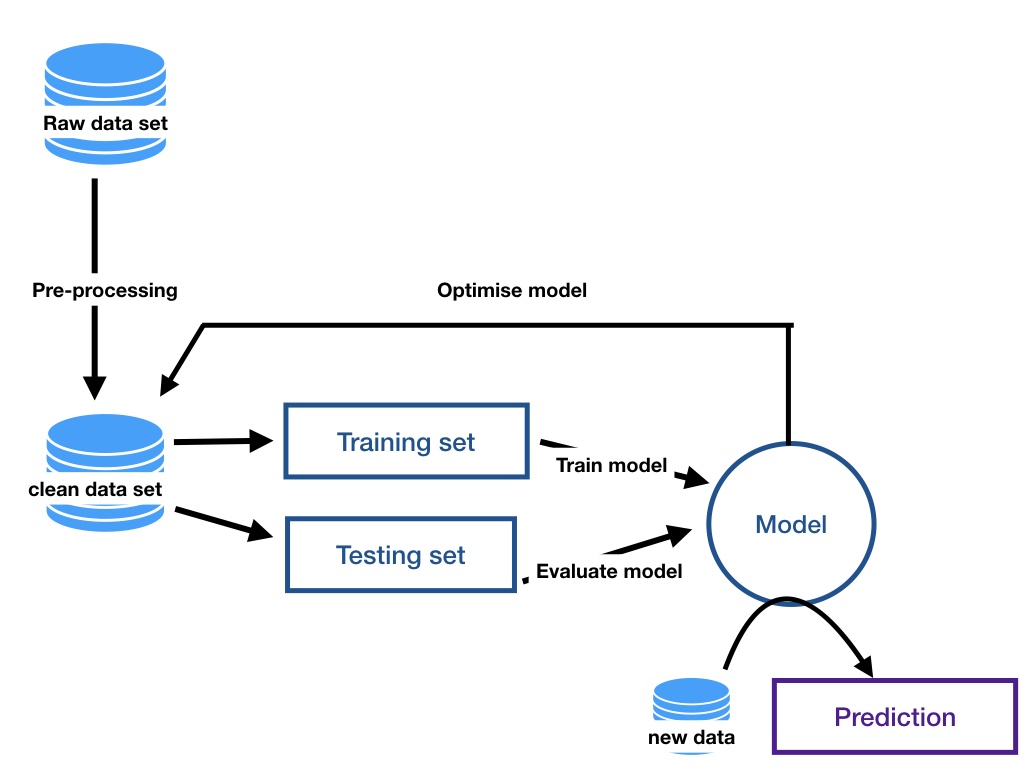
\includegraphics[width=0.8\textwidth]{ThesisTemplate/usingLatex/images/supervisedLearning.png}
    \caption{An example workflow of the supervised learning process. Pre-processing refers to any treatment of the data before it is used to train the algorithm and can include normalising, imputing or scaling.}
\end{figure}


\subsection{Evaluating Performance and challenges}

\subsubsection{Performance evaluation}
There are many ways to evaluate the performance of a supervised learning algorithms. In section 2.2.1, the TP, FP, TN and FN numbers were explained and these are used in a number of the metrics that have been developed to assess the performance of a given algorithm.

Although there are additional ways to assess the performance of an algorithm, this section will discuss the following ones: accuracy, calibration, discrimination, negative predictive value, precision, recall and specificity \citep{Callahan:2017bz}.

\begin{enumerate}
    \item Accuracy \newline
    The accuracy of a model is defined as the number of correct predictions made by the model (i.e. TP and TN) divided by the total number of predictions made.
    
    \begin{equation}
        A = frac{TP + TN}{TP + FP + TN + FN}
    \end{equation}
    
    \item Calibration\newline
    This is a measure of how closely predicted probabilities for an outcome match the observed outcome in test data, also known as the Brier score
    
    \begin{equation}
        Brier score = \frac{1}{N} \sum_{i=1}^{N} (p_{i} - o_{i})
    \end{equation}
    
    \item{Discrimination}
    Discrimination is a measure of how well a model discriminates between randomly selected true positive cases and true negative cases, usually measured as the area under the receiver operator curve (AUC).
    
    \begin{figure}[H]
    \centering
    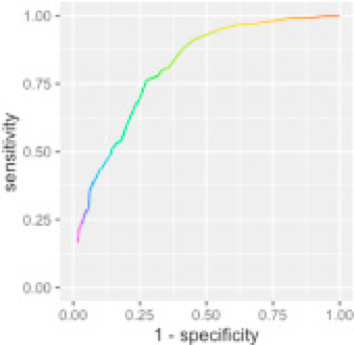
\includegraphics[width=0.5\textwidth]{ThesisTemplate/usingLatex/images/AUC.png}
    \end{figure}
    
    \item{Negative Predictive Value}
    This is obtained by dividing the total number of correct negative classifications made (TN) by the total number of negative classifications (TN + FN).
    
    \begin{equation}
        NPV = \frac{TN}{TN+FN}
    \end{equation}
    
    \item{Precision or Positive Predictive Value}
    Precision is the total number of correct positive classifications made (TP) dividided by the the total number of positive classifications made (TP + FP).
    
    \begin{equation}
        P (or PPV) = \frac{TP}{TP + FP}
    \end{equation}
    
    \item{Recall or Sensitivity}
    This metric is also known as the true positive rate and is calculated by dividing the total number of correct positive classifications made (TP) by the number of positive class members in the data (TP + FN).
    
    \begin{equation}
        R = \frac{TP}{TP+FN}
    \end{equation}
    
    \item{Specificity}
    This metric is also known as the true negative rate and is obtained by dividing the total number of correct negative classifications made (TN) by the number of negative class members in the data (TN + FP).
    
    \begin{equation}
        S = \frac{TN}{TN+FP}
    \end{equation}
    
\end{enumerate}

\subsubsection{Challenges in supervised machine learning}
\begin{enumerate}
\item{The bias-variance tradeoff:}\newline
An important concept in supervised learning is that of bias-variance trade off and the bias variance decomposition is a useful tool to understand the performance characteristics of a learning algorithm. The  mean squared error of a model is made up of the bias and the variance. Bias indicates how accurate the model is on average across different training sets. The variance indicates how sensitive the learning algorithm is to small changes in the training data \citep{Sammut:2016gd}.

\begin{equation}
        MSE = bias^2 + variance
\end{equation}

Thus, any effort to reduce the variance will increase the bias and vice versa. Typically, a model with large bias and low variance will have a tendency to overfit as shown in figure . Linear Regression, Linear Discriminant Analysis and Logistic Regression are all example of algorithms which exhibit high bias and low variance \citep{Anonymous:2016um} whereas Decision Trees, k-Nearest Neighbors and Support Vector Machines exhibit low bias and high variance \citep{Anonymous:2016um}.

\begin{figure}[H]
    \centering
    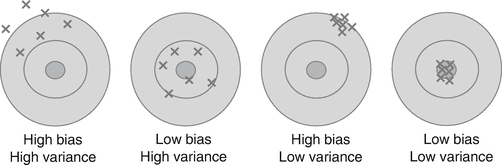
\includegraphics[width=0.8\textwidth]{ThesisTemplate/usingLatex/images/biasvariance.png}
    \caption{Adapted from \citep{Sammut:2017vv}, the optimal scenario is that of the furthest right target, although in practice this is difficult to obtain; Models displaying high bias and low variance will be more uniform but less accurate(third target) whereas models with low bias and high variance will be more accurate but less uniform. The least optimal scenario is that of a high bias and high variance.}
    \label{fig:my_label}
\end{figure}

In supervised learning, model complexity and bias-variance trade-off have to be considered and they are in fact interrelated. Typically an overly simple model with few parameters will display high bias and low variance \citep{Anonymous:vm} but a complex models with many parameters will show low bias and high variance, thus it is important to find the right balance of complexity as determined by the bias-variance tradeoff.

\item{The class imbalance problem:}\newline
A dataset is said to suffer from a class imbalance problem when the class distributions are highly imbalanced i.e. one class is greatly underrepresented \citep{Ling:2017jm}. This can lead many classifiers to have low predictive accuracy for the infrequent class. It is assumed that in a two-class case, the minority class is the positive class and the majority class is the negative class. In many real life cases (e.g. medical applications), the minority class could be as infrequent as 1\% of the dataset, thus is a cost-insensitive classifier were applied to the data, it is highly likely that the classifier would predict everything as negative. This is of particular interest in real-life applications where either the goal of the classifier is not to maximise accuracy or the class distribution of the training and test sets are very different \citep{Ling:2017jm}.\newline
If the cost of different types of error (i.e. that of False Positive versus that of False Negative) for a classifier is not the same a cost-sensitive learning algorithm can be used instead \citep{Ling:2017jm}.\newline
In the case of different class distribution between the training and testing data, one approach can to sample the training data in such a way that its class distribution matches that of the test data; this can be achieved by oversampling of the minority class and undersampling of the majority class. \newline
Another approach is to split the minority and majority class into sub classes that relate to the original classes. For instance if the majority class was Healthy (H) and the minority class Sick (S), they could be further divided as VH (very healthy), H and BH (borderline healthy) and BS (Borderline sick), S and VS (very sick). This implies a good knowledge of the domain but has the advantage that LS, S and VS are all scored as positive and VH, H and BH are all scored as Healthy, which may improve the accuracy of the algorithm by reducing the class imbalance (Eyad Elyan, personal communication).
\end{enumerate}

\section{Machine Learning in Healthcare}
\subsection{Motivation: data in healthcare}
One key area where machine learning is being invested in is the healthcare sector \citep{Obermeyer:2016ju,EMC:2014ve, Evans:sHGdqFvY} and see figure 2.2. Indeed data growth in this sector has been growing at a faster rate than other sectors (48\% annual growth versus 40\% growth on average for other sectors) according to a report from EMC \citep{EMC:2014ve}. And it is thought that new healthcare applications will drive data growth. For example, the adoption of Electronic Health Record (EHR) in the United States by healthcare providers (hospitals, GP) is growing so fast that it is estimated that by 2020, penetration of EHR in the US market will reach 95\%. Further, increasingly stringent regulations of data protection and maintenance, especially in the healthcare sector means that many providers choose to keep data indefinitely \citep{EMC:2014ve}.  However large amounts of this data is still largely unused and according to the EMC corporation, better data analytics will help identify the most useful data, which will in turn enable information-driven decision.
The healthcare sector also faces challenges in most parts of the world. Firstly, the global population is ageing. According to data collected by the United Nation Department of Economic and Social Affairs (Population Division), the number of older persons (60 years or over) is estimated to more than double by 2050, rising from 962 million globally in 2017 to 2.1 billion in 2050, meaning that population aged 60 or over is growing faster than all younger age groups \citep{UnitedNations:2017wd}. An ageing population with longer life expectancy will make more demands on the health services everywhere. A second challenge of the sector is the shortage of physicians and other care providers. For example in the United States, the number of primary care physicians is expected to increase by only 8\% whereas the demand for primary care physicians will rise by 14\% resulting in a shortfall of around 20, 400 physicians \citep{EMC:2014ve}. The trend is similar in the UK and other European countries \citep{Campbell:ti}. At the same time, patient expectations will increase as people will expect treatments and care in line with technological developments.\newline
Together these factors  mean that the healthcare sector needs to adapt and to be able to deliver care in the most efficient way and will need to turn to Information Technologies in general to help scaling the process, and to machine learning in particular in order to facilitate a greater output of robust diagnosis, uncover novel drug candidates, or detect best possible treatment given a patient's background.\newline

\subsection{Opportunities for the use of machine learning in healthcare: what problems can be solved?}
Although the use of machine learning in healthcare is not new (there are many commonly used teaching healthcare-related datasets from studies done in the 1980s and 1990s; the Breast Cancer Dataset for example was first used in a study published in 1994 \citep{OLMangasarian:1994ue} and the Pima Indian Diabetes dataset was used in a study from 1988 \citep{Smith:1988wy}), recent years have seen an increase in publications relating to machine learning and healthcare, most likely driven by the general growth in machine learning centred research as discussed in the previous section but also by the increasing volume of data being produced \citep{Pesapane:2018kv}. Figure 2.5 shows the increase in publications which were found in EMBASE by using terms such as machine learning or deep learning and radiology, showing an 8-fold increase since 2006. A search in Google Scholar with the terms "Machine Learning" and "Healthcare" for articles published between 2016 and 2018 returned 978 results.\newline

\begin{figure}[H]
\centering
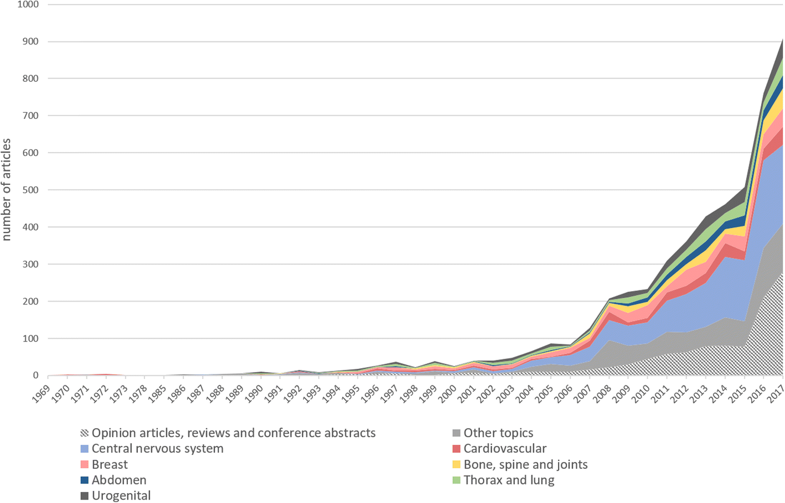
\includegraphics[width=0.7\textwidth]{ThesisTemplate/usingLatex/images/PesapaneFig.png}
\caption{Figure from \citep{Pesapane:2018kv}: Number of publications indexed on EMBASE obtained using the search query ('artificial intelligence'/exp. OR 'artificial intelligence' OR 'machine learning'/exp. OR 'machine learning' OR 'deep learning'/exp. OR 'deep learning') AND ('radiology' OR 'diagnostic imaging'). EMBASE was accessed on April 24, 2018. For each year, the number of publications was subdivided separating opinion articles, reviews and conference abstracts from original articles in seven main subgroups considering subspecialty or body part. Other fields of medical imaging different from those listed above are grouped under the “other topics” label (e.g. dermatology, ophthalmology, head and neck, etc.)}
\end{figure}

The previous chapter discussed briefly the potential of machine learning to greatly help in the field of epidemiology by providing an alternative to randomised control trials (RTC) or case-control studies by exploiting large patient datasets which are now available in electronic format across large geographical areas \citep{Callahan:2017bz}, through the adoption of EHR. Studies where machine learning has been applied to EHR are increasingly popular \citep{Goldstein:2017bk}.\newline 
EHR data differs from to traditional cohort based risk-studies since the data may not be standardised, is generally collected more frequently and is collected without the use strict inclusion requirements. 
There are advantages to the use of EHR data as they are typically collected more often than those from cohort studies and will more often reflect real-world situations than the data obtained from restrictive cohort studies. In one such case, a model to predict heart failure survival was built using EHR data from the Mayo Clinic \citep{Panahiazar:2015gp}. The authors compared their model to the existing Seattle model and found that the use of EHR data provided a model that was more accurate (11\% AUC improvement) and more convenient to use in clinical setting. Panahiazar and colleagues suggested that one of the reason their model showed better predictions than the existing one is that the Seattle Heart Failure Model (SHFM) is extrapolated from clinical trial databases and therefore does not always reflect real-life situations.
There are many more areas where machine learning could improve healthcare delivery such as the stratification of patients into risk category or to characterise and predict a variety of health risk, as well as early diagnostic of certain condition. The literature abounds with examples of successful machine learning algorithms which have been developed with these goals in mind. \newline 
Traditional risk scoring system can be flawed as some of the features used to compute the score may not reflect a wide enough variety of the population \citep{Besseling:2017bs}. Those limitations have led several group to turn to machine learning to build robust statistical models that will classify individuals appropriately and provide accurate level of risks \citep{Callahan:2017bz, Besseling:2017bs}.\newline
Several research groups have successfully developed algorithms that outperformed existing stepwise logistic regression models to predict the risk of mortality of an individual or to diagnose a condition in a patient. For instance  Ross and colleagues developed a machine learning algorithm to identify the presence of peripheral artery disease (PAD) and predict future mortality risk \citep{Ross:2016kh}.The data used in this study was derived from a prospective observational study with a view to identify key demographic, clinical and genomic factors that differs between those presenting with PAD and those that do not. The disease was not used as a factor for enrolling patient in the study, however patients enrolled included those referred for complaints of angina, dyspnea or had abnormal stress results. Clinical data were obtained at enrolment and patients were followed for observation of any adverse event. Therefore there is a small element of bias in the sample used to build the algorithm, although the presence of PAD was not known at enrolment, the patients were already being enrolled in a study because of a number of complaints. \newline
 To build the model, the researchers included any variable for which a majority of patient had a data value. In other words, no variable was included based on \textit{a priori} hypotheses and patients were included if they had complete data. The researchers were able to build a Random Forest-based algorithm that successfully identified undiagnosed PAD (AUC:0.84). The model was also used to predict mortality (AUC:0.76). PAD is highly prevalent as well as difficult to diagnose, so this algorithm could prove very useful in a clinical setting.\newline
 Despite the algorithm performance, there are several limitations to this study. Firstly the algorithm was constructed using only those patients with complete data. This is problematic for clinical application, as patient records are often incomplete (as discussed previously) for a variety of reasons. The authors suggest the possible imputation of data in cases of missing values \citep{Ross:2016kh}. As previously mentioned, the population used to train the algorithm is already considered  to be high-risk, thus the algorithm may not generalise well to other populations. \newline
 Other efforts at patient risk classification have been made  and by other groups have included the application of machine learning to the selection of individuals for genetic testing for familial hypercholesterolemia (FH) \citep{Besseling:2017bs} in an attempt to improve current selection criteria which tend to misclassify certain population, especially young individuals.\newline
 The work carried out by Besseling and colleagues provided a useful model which showed good discrimination and calibration, which compared to existing models allowed for better inclusion of young persons (which the previous models tended to exclude) and this new model is being considered for use in clinical setting. This work allows for the selection of individual for genetic testing which is often expensive and therefore needs to be targeted. The model is to be used on patients with suspicion of FH rather than the population at large.\newline
 Other areas of healthcare where machine learning has been successfully applied include imaging diagnostic, as early as 1994 \citep{OLMangasarian:1994ue} and more recently Aissa and colleagues investigated the impact and clinical performance of a machine learning based tool for the detection of lung nodule in melanoma patients \citep{Aissa:2018jm}. \newline
 The diagnostic of lung nodules is one of the criteria to identify metastases in cancer patients as well as being used for screening of primary malignancies of the lung. The presence of lung nodules in melanoma patients the presence of pulmonary metastatic disease is an indicator of worsen prognosis so its accurate identification is important. In this study the authors compared the reading of CT scans by three radiologists to that of a computer aided detection system (CAD). This novel CAD system is machine learning based and the additional vessel-suppressed reconstruction can be viewed by the radiologist. \newline
 The CAD system did not miss any of the nodules identified by the radiologists also reviewing the images, however the system found additional nodules, which were missed by the radiologists. These turned out to be very small and did not affect therapy. In 9\% of these cases, theses nodules turned out to be false positives and follow up analyses revealed that none of the nodules detected by CAD but missed by radiologist were metastases or would have led to changes of therapy. In 30\% of the cases where the nodules where missed by the radiologist, they were so small that they could not be definitely labelled as benign or not, which means patients needed to be further referred for follow-up. This could lead to further follow-ups and increased costs as well as patient distress. This study suggests that machine learning aided diagnostic can be of great help particularly in cases where early detection of disease is crucial to patient survival, but the authors stress that findings need to then be reviewed by the appropriate specialists (in this case radiologist) in order to be appropriately interpreted and the CAD system should be used as either second reader or concurrent reader. It is worth noting that the study concerned only a relatively sample size (46 patients) and larger sample sizes may have shown a different false positive result, or the presence of nodules missed by either the CAD system or the radiologists.\newline
 The studies discussed above all show that machine learning can be a powerful tool for diagnostic medicine although there are limitations inherent to the study design or the choice of dataset and these are discussed in section 2.4.\newline
 As previously shown in figure 2.5, Diagnostic Imaging has been a centre of interest for the application of machine learning tools to assist radiologists in their tasks. William and colleagues conducted a review of image analysis and machine learning techniques used for automated cervical cancer screening \citep{William:2018ia}. In total, they reviewed 30 publications from the last 15 years and found that most of the existing algorithms facilitate an accuracy of nearly 93.78\% on an open pap-smear data set, segmented using CHAMP digital image software. K-nearest-neighbors and support vector ma- chines algorithms have been reported to be excellent classifiers for cervical images with accuracies of over 99.27\% and 98.5\% respectively when applied to a 2-class classification problem. \newline 
 This review identified some weaknesses in the techniques used, including low accuracy of classification in some classes of cells. Most algorithms documented either worked on single cervical cell images or multiple cervical smear images not both, the authors suggested that algorithms that can be used on both single and multiple cell images at the same time should be investigated as cells in pap-smear images usually contain overlapping cells.\newline
 The authors also reported that the majority of the algorithms resulted in an accuracy of nearly 93.78\% (still low for diagnostic purposes) and used an open pre-processed pap-smear data set, suggesting that the accuracy of these algorithms could be even lower in a clinical setting, using images that have not already been processed.\newline 
Other areas of the healthcare industry where machine learning could also be useful are numerous and include hospital and practice management, for example to predict demand for emergency department beds or to inform staffing decision \citep{Callahan:2017bz, Tiwari:2014bq}. These applications have the potential to be useful especially in environment for resources are scarce and they present challenges quite different to those centred around patient diagnostic or disease risk predictions. For the purpose of this review, this aspect of machine learning in a healthcare setting will no be discussed further and is only mentioned here for indicative purposes.


\section{Challenges in healthcare}
\subsection{Challenges inherent to the data}
The use of machine learning as applied to healthcare related data is not without challenges. 
Electronic health record data present some difficulties as EHR data is captured for all patients mostly when they are unwell and collect only those metrics that the clinician will think is appropriate for a particular visit, and this can introduce bias in the data \citep{Hersh:2013gp, Goldstein:2017bk}. \newline 
Goldstein and colleagues looked at a large number of EHR and machine learning based studies and analysed both their methodologies and result to  establish areas of weakness and suggestions for future studies to remedy those problems. They identified four main areas where improvements were necessary in order to get the best possible results for EHR based studies: 
\begin{itemize}
    \item Many studies were not carried across multiple centres or did not cross validate using data from another centre, which does not guarantee the portability of the model 
    \item Predictor variables were not always used to the fullest extent of the EHR data and better leverage from the available information could be gained by using time-varying factors
    \item Bias inherent to the data (EHR data contains sicker people on average) is not always addressed which could in turn affect the robustness of the model
    \item Evaluation metrics were often not suited to the data or the model (c-statistic) and should instead have used Predictive Positive Value or Net benefit metrics. 
\end{itemize}

Conversely, although EHR data tend to be biased towards a higher rate of sick patients, many health-related dataset can be biased towards healthy patients, especially when using cohort-based data. In this case, there are only a small subset a patient with the disease or marker that is being investigated and this can lead to developing models that will easily fail to identify the targeted outcome because the training sets do not contain enough instances of the "sick" label compare to the "healthy" label. This is known as the class imbalance problem and was discussed in section 2.2.2. 
As discussed earlier, this problem can be resolved through stratification of the data or changing from a binary category to a multiple category.
Another common challenge from working with health-related dataset is the problem of missing data. It is especially common when working with EHR \citep{Goldstein:2017bk} but can also happen when working with cohorts and this problem was discussed in several of the examples discussed previously \citep{Besseling:2017bs, Ross:2016kh}.\newline
Both studies resorted to data imputation \textit{i.e} the process of replacing missing data with substituted values. This is often done by replacing the missing values with the median value for that variable. Ross and colleagues even report, although this is not published that imputation of missing data may improve predictive accuracy \citep{Ross:2016kh}.\newline
In the studies described in section 2.3, there were several methodological considerations and limitations that were taken into account by the authors. The inclusion or not of variables towards the final model is one such consideration. Often a stepwise selection, without considering previously known association between candidate predictors and outcome, is used. However this might exclude variables that appear statistically insignificant in a multivariable model but would be significant when used in another cohort and may therefore impact the portability of the model. In contrast, by using only variables that have been previously shown to contribute to the outcome while ignoring those that show association in the data, the model risk missing important associations that are yet to be identified \citep{Besseling:2017bs}. To avoid either of these pitfalls, Besseling and colleagues chose to use a two-step approach in choosing the candidate predictors: 
 \begin{itemize}
 \item firstly all variables considered important (based on current literature regarding clinical phenotype of FH) were included in a preliminary model;
 \item then the authors added a combination of eight variables to the model, with a maximum of four added at any time.
\end{itemize}
In contrast the model to identify PAD described by Ross and colleagues \citep{Ross:2016kh} was built by using all variables for which data was available so as to limit deliberate bias in choosing which variables to include in the model.\newline
The size of the dataset used for a study is also of notable considerations as smaller dataset can lead to bias and overfitting  of the data \citep{Steyerberg:2003fq}. Though many studies using machine learning use large datasets, many fail to use multiple centres which may reduce the utility of the model when extrapolated to different population and this has been noted by Goldstein and colleagues \citep{Goldstein:2017bk}. The familial hypercholesterolemia model built by Besseling and colleagues successfully avoided this pitfall using a large training dataset and using an external validation set from a different cohort \citep{Besseling:2017bs}. In the case of the PAD model study, the authors acknowledged that their training size was relatively small and from patients that had been chosen because their data were complete and this could limit use of the model in a clinical setting \citep{Ross:2016kh}.\newline
This also raises another challenge that occurs when developing machine learning in healthcare is that of class distributions being very different between the training dataset and the testing datasets. In the case of the study on Familial Hypercholesterolaemia, the algorithm was validated using a testing set that was unrelated to the training set, though the class distribution were similar between the two sets and the two classes were fairly evenly distributed in both sets (40\% and 60 \% in the training set and 45\% and 55\% in the testing set) \citep{Besseling:2017bs}. However, this could be very different in a clinical setting or if the algorithm were to be expanded to a different population where it might be expected the gene mutation may be more or less frequent than in the one used to develop the algorithm. William and colleagues also cites this as a potential problem with many of the algorithms they have reviewed \citep{William:2018ia} since they were trained on commercially, pre-processed images rather than ones obtained from hospitals or clinics.


\subsection{Data access}
Patient level data is considered sensitive data and is therefore protected. In the UK it falls under the Data Protection Act \citep{Anonymous:YZCGtNyR}  and there are similar laws in place across many other countries.\newline
In order to use patient level data for research purposes, consent of each patient has to be obtained, unless the data is processed so as to be anonymised and collated in such a way that no individual patient can be  identified from their data. In the UK, the CPRD (Clinical Practice Research Datalink, https://www.cprd.com) is responsible for collecting de-identified data from a network of GP practices. This data can be accessed by research groups through an application process \citep{CPRD:VYxcqU74}. Other de-identified data are released by NHS digital for NHS England and by Information Data Service for NHS Scotland.
Other collected-for purposes data can be obtained in the same way as they are obtained for clinical trials. A number of datasets that have been used for published research have now been placed in a de-identified format in the public domain through organisation such as Kaggle(https://www.kaggle.com) or UCI(http://archive.ics.uci.edu/ml/index.php). Many datasets relating to healthcare can be found on these websites and used to create new algorithms or compare the performance of different algorithms on specific datasets.\newline
There are a growing numbers of wearables (Apple Watch, Fitbit, etc) that collect health-related individual data, however these tend to be protected by data protection laws and the various private companies in charge of hosting the data may not share them with researchers unless consent has been explicitly seeked from the user \citep{Apple:nN4TDuuN, Fitbit:FvPrmdk3}. Finally, there has been growing enthusiasm from the public in genomic level data and for profit organisation such as 23AndMe or Ancestry have seen a growing number of customers looking to find out more about their disease risk or ancestry through DNA testing \citep{Regalado:vf}. These companies have various consent policies and will either not share the data or will seek consent of the consumer to share data with selected partners only. 


\subsection{Cultural Challenges: response from healthcare staff and patient}
Although the use of machine learning in the healthcare sector appears to be growing at least in a research setting, its full implementation in clinical setting is still facing some opposition from providers \citep{Cabitza:2017hv}. Though some view the growing use of AI and machine learning in healthcare as inevitable \citep{Murdoch:2013hm} and there are advocates for opening data use in healthcare \citep{Kostkova:2016ur}, with many viewing it as tool which can support rather than replace medical providers \citep{Pesapane:2018kv}.
Although there are some reticences from patient in sharing their health data for research purposes \citep{Goldacre:tf}, there is evidence that these attitudes may be shifting \citep{Kostkova:2016ur}. 

\section{Conclusions}
This chapter has reviewed the existing literature relevant to the use of machine learning in the field of healthcare, although the review is in no way exhaustive and has concentrated on aspects of medical diagnostics rather than healthcare management or planning. 
The current level of research in the application of machine learning to healthcare has been increasing in the last decade and the work reviewed in this chapter suggests that machine learning could help the healthcare industry solve some of its staff shortage issues through the partial automation of some of its diagnostic procedure (particularly in the field of imaging). Machine learning could also solve problems in providing patient with the necessary care at the earliest possible time for a given condition through the development of more accurate risk scoring systems. Finally, machine learning could assist with leveraging the ever increasing volume of data generated in the healthcare sector.\newline
These objectives are not without challenges however and the use of machine learning in assisting medical diagnostic can only succeed if those challenges are recognised and addressed appropriately.
First there are some bias inherent to the data used in healthcare-related studies and these bias need to be addressed during data pre-processing if helpful models are to be developed. Investigating possible solutions to the problem of class imbalance and comparing different way to pre-process the data through feature engineering or other methods may be avenues to improve the performance of algorithms on this type of data.  \newline
Second access to data can be difficult. The development of algorithms using open datasets or carefully recruited cohorts may not yield models that can be deployed across larger populations in a clinical setting and it will be necessary to tap into both EHR data and data obtained from wearables and/or privately requested genomic data through initiatives so that algorithms can be trained on large cross-section of the population.
\newline
A third category of problem broached while reviewing the literature and relating to data access is the issue of consent to use of data, data protection and more generally health provider and patient attitude toward the use of machine learning in healthcare, however this falls outwith the scope of this project and will not be discussed further. 





\chapter{Design}\label{ch:Design}

\section{Introduction}
\subsection{Problem Definition and outline}
In many types of datasets, a class imbalance is frequent as there are much fewer incidences of the target outcome label than of the "normal" ones . Class imbalance in data  can lead algorithms to misidentified instances, giving a "normal" label to a target instance, for example, because the data on which the algorithm was trained did not contain enough instances of the "target" label.  There are many real-life instances where the wrong classification of an instance could have devastating consequences and the aim of this project is to:
\begin{enumerate}
\item compare the performance of several different algorithms on imbalanced datasets
\item identify potential solutions that will allow the algorithms to "learn more efficiently" even when a class is underrepresented
\item test the different solutions and compare the performance of the algorithms on the same datasets once the solutions have been implemented
\end{enumerate}
\subsection{Class Imbalance in healthcare datasets}
Healthcare-related datasets are particularly sensitive to the class imbalance problem and this can be more or less severe depending on the condition that is being studied. Some diseases have a more frequent occurrence than others, for example certain types of cancer have a very low incidence, especially when looking at the general population, while others are much more common, though their incidence in the population at large will still create a class imbalance. There are however situations where the class imbalance is reversed and incidence of "sickness" tends to be higher than that of "health", and this has been reported in EHR data; since EHR data are formed from doctors' patient records, there tends to be an over-representation of unhealthy cases versus healthy ones in those dataset. In either case, the intrinsic bias of the data towards one of the classes will create issues when training an algorithm as there are insufficient cases of one class to learn from. This will likely result in the algorithm failing to identify properly cases of "sick" label for example and mislabelling them as "healthy". This problem could be further amplified if the class distribution in the data used for training is very different from the class distribution in the testing or live data, on which the algorithm will be used.
In cases of medical diagnosis this could have dramatic consequences as the wrong diagnosis could be issued to a patient. 


\subsection{Experimental design outline}


\begin{figure}[H]
    \centering
    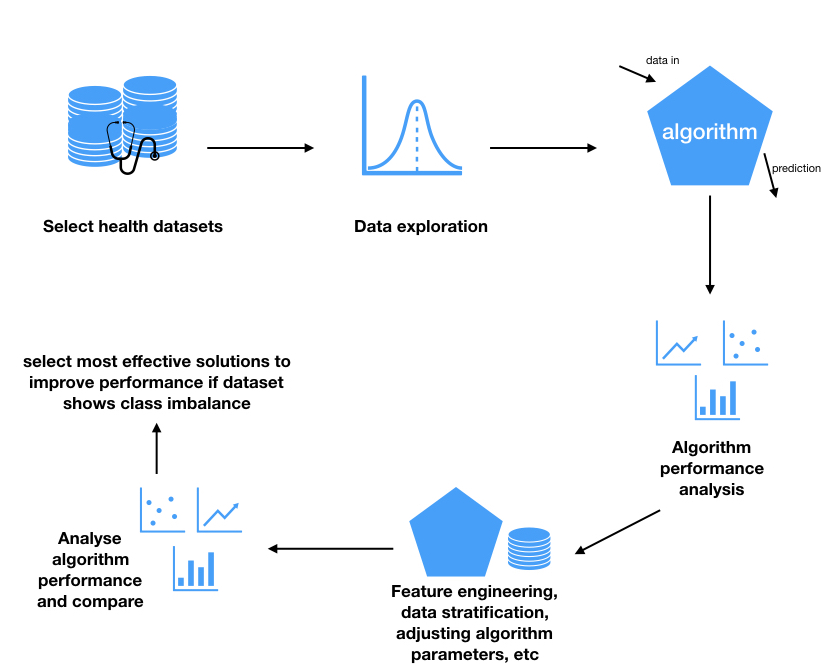
\includegraphics[width=0.8\textwidth]{ThesisTemplate/usingLatex/images/Chapter3Figures001.jpeg}
    \caption{Schematic of the experimental design of the study.}
    \label{fig:expDesign}
\end{figure}

\section{Dataset Choice and Preliminary Exploration}
\subsection{Datasets}
\subsubsection{How were the dataset chosen?}
The Kaggle repository of datasets (https://www.kaggle.com/datasets) was searched for datasets with the tags "healthcare", "health", "oncology and cancer" and "health sciences".
This search returned 223 datasets. Genomic/proteomic datasets were discarded as they are best suited to clustering tasks. Datasets where classification tasks could be carried out were kept and further examined.
A total of 9 datasets were retained for use in the analysis.

\subsubsection{Brief Overview of the datasets}
The datasets chosen for the analaysis were:
\begin{itemize}
    \item Breast Cancer Wisconsin Data Set\footnote{https://www.kaggle.com/uciml/breast-cancer-wisconsin-data}  
    \item Indian Liver Patient Records\footnote{https://www.kaggle.com/uciml/indian-liver-patient-records} 
    \item MRI and Alzheimers \footnote{https://www.kaggle.com/jboysen/mri-and-alzheimers\#oasis\_longitudinal.csv}
    \item Pima Indian dataset\footnote{https://www.kaggle.com/uciml/pima-indians-diabetes-database} 
    \item Cervical Cancer Risk Classification\footnote{https://www.kaggle.com/loveall/cervical-cancer-risk-classification  }
    \item Lower back pain symptom dataset\footnote{ https://www.kaggle.com/sammy123/lower-back-pain-symptoms-dataset}
    \item Heart Attack Prediction\footnote{https://www.kaggle.com/imnikhilanand/heart-attack-prediction}
    \item Autism Screening\footnote{https://www.kaggle.com/faizunnabi/autism-screening/home} 
    \item Fertility dataset\footnote{https://www.kaggle.com/gabbygab/fertility-data-set} 
    
   
\end{itemize}

All 9 datasets allow classification tasks to be carried out, most of them on a binary basis.

\subsection{Class distribution of the datasets}
Table 3.1 sums up the class distribution for the datasets chosen. The class distribution is written in the format HealthyValues - OutcomeValues.
As can be seen from the table, not all datasets have similar class distribution, though most of the selected ones have a 25-25\% of the Outcome class apart from the Autism set and the cervical cancer set which have less than 10\% of the data representing the target class. \newline This range of class distribution will provide interesting case studies to compare the effect of class distribution on the performance of various algorithms. It could also be possible to artificially manipulate the testing data after the split of data by removing instances of the target class so as to mimic real world incidence of the conditions represented in the datasets. In doing so, the performance of various algorithms could be measured on testing sets that are more realistic.

\begin{table}
\begin{tabular}{ p{4.5cm}p{1.5cm} p{1.5cm}  p{2 cm} p{1.5cm}}
 \hline
 \multicolumn{5}{c}{Datasets} \\
 \hline
 \hline
 \rowcolor{LightCyan}
 Dataset Name & Instances & Columns & Class Distribution & \% Minority Class \\
 \hline
 Breast Cancer Wisconsin Data Set& 569 & 32 & 
357-212 & 37.0\\
Indian Liver Patient Records&  583 & 11  & 416-167 & 28.0 \\
Pima Indian dataset& 768 & 9  & 503-265 & 34.0 \\
Cervical Cancer Risk Classification & 858 &  36 & 802-56 & 6.52\\
Lower back pain symptom dataset & 310 & 13  & 101-209 & 67.4\\
Heart Attack Prediction & 294 & 14  & 188-106 & 36.0\\
Autism Screening&704 & 21 &514-90 & 1.2 \\
Fertility dataset&100  & 10 & 89-11 & 11.0\\
\hline
\end{tabular}
\caption{Summary of datasets chosen for the analysis}
\label{tab:1}
\end{table}


\section{Choice of algorithms used in evaluation}
\subsection{Quick overview of algorithms}
This works focuses on supervised learning classification tasks. Several supervised machine learning algorithms have shown promises in computer-aided diagnosis (CAD) \citep{Dua:2014dz}:
\begin{itemize}
    \item decision trees (DT) such as Random Forest are easy to comprehend and relatively easy to implement but are challenging to apply to non linear problems \citep{Gray:2013eh}
    \item support vector machine (SVM) \citep{Naraei:ct}
    \item k-NN \citep{Liu:2011dz}
    \item Bayesian models \citep{Dangare:ut}
\end{itemize}

\subsection{Reasons for choosing those algorithms}
The algorithms listed above have demonstrated high performance in classifying tasks on healthcare data, even in the case of imbalanced datasets \citep{Dua:2014dz}. They also utilise different mathematical approaches to classification and therefore are expected to behave differently from one another.



\section{Proposed avenues of exploration}
\subsection{Overview of typical methods to address class imbalance}
The class imbalance problem was discussed in chapter 2 along with some of the techniques used to compensate for its effects. These techniques are discussed here further and can be separated in data-level solutions and algorithm-level solutions:
\begin{enumerate}
    \item Data-level solutions\citep{Sun:2013it}
    \begin{itemize}
        \item undersampling the prevalent class 
        \item oversampling the minority class
        \item detecting the sub-concepts constituting a class and  oversampling each concept to balance the overall distribution
    \end{itemize}
    \item Algorithm level solutions
    the solutions here are highly dependent upon the algorithm and in order o develop an algorithmic solution, knowledge of the classifier learning algorithm and the application domain is necessary as well as a thorough comprehension on why the learning algorithm fails when the class distribution of available data is uneven
    \begin{itemize}
        \item choosing an appropriate inductive bias (e.g. for decision trees, adjusting the pruning technique)
        \item for SVMs, different penalty constants can be used for different classes
    \end{itemize}
    \item Cost-sensitive learning\citep{Sun:2013it}
    Cost-sensitive classification considers the varying costs of different misclassification types i.e. various penalties are applied for classifying one class as another. In this situation, the learning aims to minimize high cost misclassifications and the total cost of misclassification.
    Cost-sensitivity can be obtained through:
    \begin{itemize}
        \item weighting the data space
        \item making a classifier cost-sensitive by adjusting parameters to minimize the cost of misclassification
        \item using Bayes Risk Theory to assign each sample to its lowest risk class
    \end{itemize}
\end{enumerate}
\subsection{Testing the Impact of the use of these methods}
\subsubsection{First test the algorithms on the dataset without any modifications}
In the first instance, all of the algorithms will be applied to all of the datasets without parameter optimisation. The performances will be noted (see section 3.5.1). 

\subsubsection{Applying the methods to each datasets and algorithms}

Then the methods discussed in section 3.4.1 will be employed on all of the datasets and the algorithms will be applied to the modified data again so that performance can be compared.\newline 
In the case of the cost-learning solutions, the parameters of the different classifiers will be adjusted so as to reduce cost of mi-sclassification, before the performance on each dataset is measured again.

\subsubsection{Testing the performance on more realistic datasets}
As an added investigation, the testing data (and potentially training) could be modified to reflect actual incidence of the conditions being observed "in the wild" and the performance of the classifiers could be tested again using the optimised parameters and methods used previously.

\section{Evaluating the performance of classifiers and of correction methods}

\subsection{Metrics for evaluation}  
The metrics to measure the performance of an algorithm have already been reviewed in section 2.2.2. and will be briefly restated here
\subsubsection{Accuracy}
This is the percentage of correct predictions made by a model and is not considered to be a good measure to use when studying highly imbalanced datasets.


\subsubsection{Confusion Matrix}

The confusion matrix describes the complete performance of the model as can be seen on figure. The number of true positives, true negatives, false positives and false negatives are all shown in the confusion matrix.

\begin{figure}[H]
    \centering
    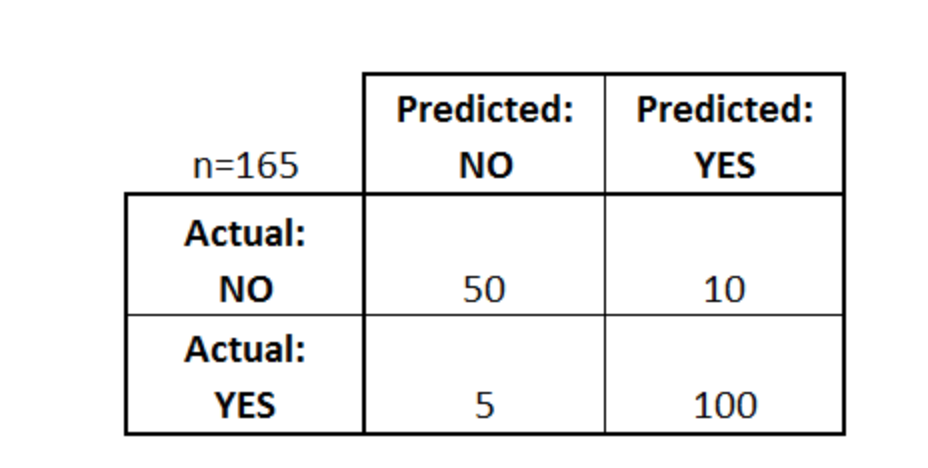
\includegraphics[width=0.5\textwidth]{ThesisTemplate/usingLatex/images/ConfusionMatrix.png}
    \caption{Metrics to Evaluate your Machine Learning Algorithm (Adapted from Mishra, A.,TowardsDataScience.com)}
    \label{fig:metrics}
\end{figure}

\subsubsection{Area under the curve}
This reflects the probability that the classifier will rank a randomly chosen positive example higher than a randomly chosen negative example. Its value is expressed between 0 and 1 (the closer to 1 the better the performance).


\subsubsection{F1 score}
This measures a test's accuracy and is obtained by calculating the harmonic mean between precision and recall. It reflects the classifier's precision and its robustness.

\subsubsection{Others}
Negative Predictive Value, Calibration and Specificity are also useful measures and may be used in the analysis.

\subsection{Choice of most relevant metrics}
\subsubsection{Which metrics will be most helpful in the healthcare context}
In the context of healthcare, it is unlikely that accuracy alone will be very useful; not only it is a poor metric of performance for imbalanced data but the cost of mis-classification in health matters could be extremely high and therefore, a poor metric is not suitable and would be at best indicative prior further analysis.

The other metrics discussed will all be considered and evaluated as to what constitutes the best measure for algorithm performance in this context.

\subsubsection{create a combined metric for this evaluation}
It may be useful to combine several of these metrics to get a more complete picture of how good or how poor the classifier is at identifying its target labels.

\subsection{Comparing performance of algorithms for each dataset before and after applying the methods to compensate for class imbalance}
Once the "baseline" performance of each classifier on the different datasets has been assessed by using the metrics discussed above, the same metrics will be measured on the same combinations of classifiers/data after implementations of the corrective methods. 
The resulting metrics can then be compared and the most effective method(s) can be assessed. It is expected that the methods to be applied will be more or less successful depending on the classifier and on the data rather than improving uniformly across all.

\section{Technical Requirements}
\subsection{Language}
R and Python are the most commonly used languages for data science and analytics. R provides some powerful and user friendly graphs and statistics, therefore making a good visualisation tool. On the other hand python focuses on productivity and code readability.
Python is a better choice if the data analytics and machine learning being carried out is closely linked to a development environment, whereas R has been mostly used in the area of statistics and research \citep{Willems:2015wi}.
Since this projects will not be involved in the development of an application or support an application logic, R will be used as it offers a large resource base of libraries and visualisation options.

\subsection{Software}

R Studio was used to write and compile code for this project. Microsoft Excel was also used to examine some of the raw data as tables. 
None of the datasets are very large and it was not necessary to use a distributed file system platform such as Hadoop.

\section{Discussion of results}
\subsection{Results obtained}
Results of analysis were collected after each run and analysis were repeated multiple times with the results aggregated so as to avoid variations.
The various settings of each experiment were carefully recorded so as to be aware of which parameters was used or which way the data was pre-processed prior analysis.

\subsection{Driving factors for the results}
The results were assessed and discussed to determine which combination of parameters, algorithm choice and data processing produced optimal performance, though this was also balanced with practical concerns. The various costs and benefits of each factors were discussed.


\section{Conclusions}

This chapter has outlined the experimental design for this project and in which way the results will be assessed and how will the success of the project be appraised. 
Nine health-related datasets have been chosen from publicly available sources and four algorithms will be used as classifiers on these datasets. The algorithms were chosen based on previous reported performance in the health sector. The different methods (data-level and algorithm-level) that can be applied to correct problems created by heavily imbalanced classes in health data have been discussed and their effects on the performance of the chosen classifiers will be assessed by measuring several performance metrics before and after their use.
The chosen performance metrics (AUC, confusion matrix, F1 score, etc) will be used to determine which methods are the most effective.






\chapter{Implementation}\label{ch:Implementation}

\section{Exploratory Data Analysis}
All code for the EDA detailed in this chapter can be found at:\newline https://github.com/AMacleod79/HonoursProjectCode
\subsection{Data Overview}

A total of eight health related datasets were chosen to examine the problem of class imbalance. As previously detailed in chapter 3, these datasets were publicly available on kaggle.com and having already been processed to some extent to either anonymise the data or render the data more workable.\newline
The extent of class imbalance varied across the different datasets and for some the imbalance was not very severe at all. In some cases a modified version of the dataset was created to attempt to replicate the real-life prevalence of the disease.\newline

\subsubsection{Cervical cancer dataset}
The cervical cancer dataset was obtained from kaggle.com. \newline
(see https://www.kaggle.com/loveall/cervical-cancer-risk-classification)\newline
This dataset looks at predicting cervical cancer diagnosis based on well known risk factors. Cervical cancer is a complicated diagnosis to make and as such there is not one single test to confirm it. A 'diagnosis' column was created as an average from the four possible diagnostic test used  (last four column: Hinselmann, Schiller, Citology, Biopsy ) \citep{Fernandes:2017td, Wu:2017fa}.\newline
The dataset contains 858 instances with 32 features and 4 target variables for each of the test carried out.
The exploratory data analysis carried out on this dataset can be found in the cited Github repository as CervicalCancerEDA.R.
The 32 features focus on lifestyle factors previously shown to influence cervical cancer risk in women, namely:
\begin{itemize}
    \item Age
    \item Number of sexual partners
    \item First sexual intercourse (age)
    \item Num of pregnancies
    \item Smokes (boolean)
    \item Smokes (years)
    \item Smokes (packs/year)
    \item Hormonal Contraceptives (boolean)
    \item Hormonal Contraceptives (years)
    \item IUD (boolean)
    \item IUD (years)
    \item STDs (boolean)
    \item STDs (number)
    \item STDs:condylomatosis (boolean)
    \item STDs:cervical condylomatosis (boolean)
    \item STDs:vaginal condylomatosis (boolean)
    \item STDs:vulvo-perineal condylomatosis (boolean)
    \item STDs:syphilis (boolean)
    \item STDs:pelvic inflammatory disease (boolean)
    \item STDs:genital herpes (boolean)
    \item STDs:molluscum contagiosum (boolean)
    \item STDs:AIDS (boolean)
    \item STDs:HIV (boolean)
    \item STDs:Hepatitis B (boolean)
    \item STDs:HPV (boolean)
    \item STDs: Number of diagnosis
    \item STDs: Time since first diagnosis
    \item STDs: Time since last diagnosis
    \item Dx:Cancer (previous diagnosis of cervical cancer)
    \item Dx:CIN (previous diagnosis of cervical intreaepithelial neoplasia)
    \item Dx:HPV (previous diagnosis of HPV)
    \item Dx (previous diagnosis of cervical cancer)
    \item Hinselmann (target variable)
    \item Schiller (target variable)
    \item Citology (target variable)
    \item Biopsy (target variable)
\end{itemize}

The exact meaning of each variable was not always straight forward to understand as the data was uploaded to kaggle by someone else than the original authors. The UCI repository also gives access to the data with scant details on the meaning of each column. The original work by Fernandes and colleagues \citep{Fernandes:2017td} does not clearly define each of the column and the link to the dataset from the published article now returns a 404 error. With these considerations in mind and based on other work carried out by other authors (Wu and colleagues \citep{Wu:2017fa}), the above attributes were used and a composite target variable was created (see below).\newline
An examination of the data structure showed that 27 columns were factors, with the column "smoke pack per year" showing 63 levels. The Random Forest function in R will only handle a maximum of 53 levels and therefore the data in this column needed to be manipulated to accommodate this restriction. \newline
First any missing values was replaced by the mean for the column. Next, it was found that there were a high number of discrete values between 0 and 1 for the number of pack of cigarettes smoked per year, and these were all considered as independent levels. All values that were less than 1 for this column were replaced by 0, taking the total number of levels for the column from 63 to 42, which is now manageable by Random Forest.\newline
All the other columns had a number of factor levels smaller than 53 and were left as such, however any missing value was replaced by the mean for the column in which it was found.\newline
A composite target variable calculated as a mean value of all 4 target variables (Hinselmann, Schiller, Citology, Biopsy was created and added as the last column in the dataset (rounded to 0 or 1).\newline
The pre-processed dataset was exported as a new .csv file to be used in the experimental stages of this projects (see table 4.2).
Finally the class distribution was represented as a bar chart and detailed in a table (see Figure 4.1 and table 4.3) 

\subsubsection{Breast cancer dataset}
The Breast Cancer dataset was obtained from kaggle.com. \newline
(see https://www.kaggle.com/uciml/breast-cancer-wisconsin-data) \newline
This dataset was developed with a view to train and test algorithms to determine whether a breast tumour was malignant or benign \citep{OLMangasarian:1994ue}. \newline
There are  569 instances each with 32 attributes and one target label (B for benign and M for malignant).\newline
The attributes were computed from images of a fine needle aspirate of a breast mass to describe the characteristics of the cell nuclei present in the image. The features were as follows:
\begin{itemize}
    \item Radius (mean of distances from center to points on the perimeter)
    \item Texture (standard deviation of gray-scale values) 
    \item Perimeter 
    \item Area 
    \item Smoothness (local variation in radius lengths) 
    \item Compactness (perimeter\^2 / area - 1.0)
    \item Concavity (severity of concave portions of the contour)
    \item Concave points (number of concave portions of the contour)
    \item Symmetry
    \item Fractal dimension ("coastline approximation" - 1)
\end{itemize}
The mean, standard error and mean of of three largest values (i.e. the "worst") for each of the feature was calculated and documented as a feature for each image.\newline

The exploratory data analysis carried out on this dataset is documented in the cited github repository as BreastCancerEDA.R.\newline
An analysis of the data structure showed no missing values. The target variable was expressed as B or M and was recoded to be either 0 (benign) or 1 (malignant), further the target variable was originally the second column but for ease of analysis in the next stages of the project this was moved to be the last column and renamed "Label".\newline
The modified dataset was exported as a .csv file for later use in the project (see table 4.2).\newline
Finally the class distribution of the dataset was computed and is shown in figure 4.1 with details shown in table 4.3.\newline 


\subsubsection{Liver Disease dataset}
This dataset was obtained from kaggle.com.\newline
(see https://www.kaggle.com/jeevannagaraj/indian-liver-patient-dataset). \newline
There are 583 instances of patient records with 10 attributes and one target variable to determine whether the patient is a liver patient or not \citep{Ramana:2011tn}. The attributes are various biochemical measures of liver health as well as patient specific information such as age and gender:
\begin{itemize}
    \item Age of patient
    \item Gender of patient
    \item Total Bilirubin
    \item Direct Bilirubin
    \item Alkaline Phosphatase
    \item Alamine Amino-transferase (sgpt)
    \item Aspartate Amino-transferase (sgot)
    \item Total Proteins
    \item Albumin
    \item Albumin and Globulin Ratio
    \item is patient (target label)
\end{itemize}

The exploratory data analysis carried out on this dataset is documented in the cited github repository as LiverDataEDA.R.\newline
The target label was set to 1 (not a liver patient) and 2 (liver patient), for consistency with respect to the other datasets used in this project, the data was recoded to 0 (not a liver patient) and 1 (liver patient).\newline
A check for missing data revealed only four instances missing a value in the albumin and globulin ratio. The missing values were replaced with the mean for that column.\newline
The pre-processed dataset was exported as a .csv file for later use in the project (see table 4.2).\newline
The class distribution was compiled and presented as a graph (see figure 4.1) and the details of the class distribution were shown in table 4.3.\newline


\subsubsection{Diabetes}
This dataset was obtained from kaggle.com:\newline
( see https://www.kaggle.com/uciml/pima-indians-diabetes-database)\newline
There are 768 instances of health data from female Pima Indian patients of at least 21 years of age. There are 8 attributes and one target variable. The target variable indicates whether the individual will develop diabetes within 5 years (1) or not (0). The attributes were as follows:
\begin{itemize}
    \item Pregnancies indicates the number of times the patient pregnant
    \item GlucosePlasma indicates the glucose concentration at 2 hours in an oral glucose tolerance test
    \item BloodPressureDiastolic indicates the diastolic blood pressure (mm Hg)
    \item SkinThicknessTriceps indicates triceps skin fold thickness ( in mm)
    \item Insulin2-Hour indicates the serum insulin concentration  (mu U/ml)
    \item BMI indicates body mass index (weight in kg/(height in m \textsuperscript{2})
    \item DiabetesPedigreeFunctionDiabetes is a pedigree function calculated by the original authors of the study which takes family history of diabeted into account
    \item Age records the age of the patient (years)
\end{itemize}
 The dataset was used in a study looking at the ADAP algorithm and further details about the pedigree function and other variables can be found in the article \citep{Smith:1988wy}.
 
The exploratory data analysis carried out on this dataset is documented in the cited github repository as DiabetesEDA.R.\newline
The target label was already set to 0 (did not develop diabetes within 5 years) and 1 (did develop diabetes within 5 years), so no recoding of the data was necessary.\newline
A check for missing data revealed none, and Smith \textit{et al.,} indicate that they replaced any missing data with 0 (which does not always make sense, e.g. for blood pressure). No further modification of the dataset were necessary and the pre-processed dataset was saved as .csv file for later use (see table 4.2).
The class distribution was compiled and presented as a graph (see figure 4.1) and details of the class distribution can be seen in table 4.3. 

\subsubsection{Lower Back Pain dataset}
This dataset was originally built by Dr Henrique da Mota with a view to classify patient as one of 3 class: Normal, patients with disk hernia and patients with spondylolisthesis \citep{RochaNeto:2009wp}. In a second classifying task, the two types of sufferers were grouped as one abnormal category. This dataset was first uploaded to UCI (see http://archive.ics.uci.edu/ml/datasets/vertebral+column) and then uploaded to Kaggle (see https://www.kaggle.com/sammy123/lower-back-pain-symptoms-dataset) as a binary classification task dataset (normal/abnormal).\newline
The dataset consists of 310 instances with 13 attributes (12 numeric predictors and 1 target label) as follows:
\begin{itemize}
    \item Pelvic incidence
    \item Pelvic tilt
    \item Lumbar lordosis angle
    \item Sacral slope
    \item Pelvic radius
    \item Degree spondylolisthesis
    \item Pelvic slope
    \item Direct tilt
    \item Thoracic slope
    \item Cervical tilt
    \item Sacrum angle
    \item Scoliosis slope
\end{itemize}

The exploratory data analysis for this dataset is documented in the cited github repository as LowBackPainEDA.R.\newline
For ease of reading and  manipulation, the columns names were replaced by the actual name of the predictor (removing col x from the name) and the unused column X was removed.\newline
The target label was set as abnormal or normal so the data was recoded to be 1 for abnormal and 0 for normal, in line with the other datasets. There were no missing values in the dataset.\newline
Uncharacteristically for a classification task, the abnormal class contains a higher number of instances than the normal class (see figure 4.1 and table 4.3). This is unusual and in order to observe a class distribution more in line with those seen in other datasets in this project, random sampling of the dataset was  carried out so as to create a modified dataset with more normal samples than abnormal. \newline
To obtain the new dataset, 7\% of the abnormal instances were  retained (resulting in a higher prevalence than current estimates of 1-3\% of low back pain sufferer, \citep{Jordan:2009vx}) and 100 \% of the normal instances were retained. The pre-processed datasets were saved as .csv files for later use (see table 4.2). The new class distribution is also shown on figure 4.1 with details outlined in table 4.3.\newline

\subsubsection{Heart Attack Dataset}
This dataset is a subset from a multi-centre, larger study which looked at patients with and without heart disease. The dataset was obtained from kaggle.\newline 
(see https://www.kaggle.com/imnikhilanand/heart-attack-prediction) \newline
The complete dataset appears to be available from UCI:\newline
https://archive.ics.uci.edu/ml/datasets/heart+Disease \newline 
though some of the files may be corrupted and the classification tasks of the original datasets is not binary.
The original dataset was made up of 76 predictors but in this dataset this has been reduced to 13 and a target variable:
\begin{itemize}
    \item Age (in years)
    \item Sex (1 = male, 0 = female) 
    \item Cp (chest pain type 1-4)
    \item Trestbps (resting blood pressure)
    \item Chol (serum cholesterol in mg/dl) 
    \item Fbs (fasting blood sugar >120 mg/dl, 1= true, 0 =false) 
    \item Restecg (resting ECG results - 0 = normal, 1 = ST-T abnormal, 2 = hypertrophy)
    \item Thalach (maximum heart rate achieved)
    \item Exang (exercise induced angina 1 = yes, 0 = no)
    \item Oldpeak (ST depression induced by exercise)
    \item Slope (slope of peak exercise ST segment)
    \item Ca (number of major vessels coloured fluoroscopy (0-3) 
    \item Thal (3 = normal, 6 = fixed defect, 7 = reversable defect) 
\end{itemize}

The exploratory data analysis is documented in the cited github repository as HeartAttackEDA.R.\newline
Nine column contained missing values, and those were replaced with the mean value for that column. Examination of the data structure revealed that columns "chol" (for cholesterol value) and "thalach" (maximum heart rate achieved) were factors with more than 53 levels (the maximum that can be handled by Random Forest), 154 and 72 levels, respectively. The number of levels was reduced by grouping levels into categories, as shown in table 4.1:
\begin{table}[!htbp]
\centering
\begin{tabular}{*5c}
  \hline
  \rowcolor{LightCyan}
  \multicolumn{2}{c}{Cholesterol} & \multicolumn{2}{c}{Thalach} \\
  \hline
  \hline
Level Value & New Level & Level Value & New Level\\ 
  \hline
    $<$100  & 100 & $\leq$90 & 90 \\ 
   $<$175 $\leq$150 & 175 & $>$90 $\leq$95   &  95 \\ 
  $<$200 $\geq$175 & 200 & $>$95 $\leq$100  & 100  \\ 
   $>$200 $\leq$225 & 225 & $>$100 $\leq$105 & 105  \\ 
   $>$225 $<$250  & 250 & $>$105 $\leq$110 & 110  \\ 
   $>$250 $<$275  & 275 & $>$110 $\leq$115 & 115  \\ 
   $>$275 $<$300  & 300 & $>$115 $\leq$120 & 120   \\ 
   $>$300 $<$325  & 325 & $>$120 $\leq$125 & 125   \\ 
   $>$325 $<$350  & 350 & $>$125 $\leq$130 & 130  \\ 
   $>$350 $<$375  & 375 & $>$130 $\leq$135 & 135  \\ 
   $>$375 $<$400  & 400 & $>$135 $\leq$140 & 140 \\ 
   $>$400 $<$425  & 425 & $>$140 $\leq$145 & 145\\ 
   $>$425 $<$450  & 450 & $>$145 $\leq$150 & 150\\ 
   $>$450 $<$475  & 475 & $>$150 $\leq$155 & 155\\ 
   $>$475 $<$500  & 500 & $>$155 $\leq$160 & 160\\ 
  `$>$500 $<$525  & 525 & $>$160 $\leq$165 & 165 \\ 
   $>$525 $<$550  & 550 & $>$165 $\leq$170 & 170 \\ 
   $>$550 $<$575  & 575 & $>$170 $\leq$175 & 175 \\ 
   $>$575 $<$600  & 600 & $>$175 $\leq$180 & 180 \\ 
                  &     & $>$180 $\leq$185 & 185 \\ 
                  &     & $>$185 $\leq$190 & 190 \\ 
   \hline
\end{tabular}
\caption{Grouping of levels for columns "chol" and "thalach" (Heart Disease Dataset)}
\end{table}

The target label was already set as either 0 (no heart disease) or 1 (heart disease) so this did not need to be modified. The modified dataset was save as a .csv file for further use in the project (see table 4.2).\newline
The class distribution is shown on Figure 4.1 and detailed in table 4.3.\newline
This dataset is fairly balanced (65:35 majority:minority). In order to create a more imbalanced dataset, random sampling of the data which will retain all of the "normal" cases and only 10\% of the "positive" cases was carried out. The modified dataset was saved for future use in the project (see table 4.2). The new class distribution is also shown in figure 4.1 (with breakdown in table 4.3) and reflects real-life prevalence of heart disease in the UK (6.7\% in men and 4.2\% in women) \citep{NHS:2018wa}\newline

\subsubsection{Autism dataset}
The Autism dataset was obtained from kaggle.com:\newline
https://www.kaggle.com/faizunnabi/autism-screening\newline
This dataset examines the predicting factors for someone to have autism or not, based on 10 behavioural features and 10 individual characteristics. The dataset was originally created by Thabtah and colleagues and further details can be found in their various publications \citep{Thabtah:2018ck}.\newline
There are 704 observations with 21 attributes and 1 target variable (does the patient have autism or not):\newline
\begin{itemize}
    \item A1 Score 
    \item A2 Score
    \item A3 Score 
    \item A4 Score
    \item A5 Score
    \item A6 Score
    \item A7 Score
    \item A8 Score
    \item A9 Score
    \item A10 Score
    \item Age
    \item Gender
    \item Ethnicity 
    \item Jundice (born with jaundice or not)
    \item Autism (relative with PDD or not)
    \item Country of res
    \item Used app before (used the screening app before)
    \item Result (score to the questionnaire)
    \item Age desc (under 18 or not)
    \item Relation (questionnaire filled by self or other)
    \item Class/ASD
\end{itemize}

A1 to A10 score represent the answer to each of the 10 question (binary) of a questionnaire for screening based on behaviour. 
The class label for this dataset is No (for not autistic) and yes (for autistic), so the data was recoded to be consistent with the other datasets to 0 for No and 1 for Yes.\newline
There were some missing values for the age column which were replaced with the mean value for the column. The "na" values for the ethnicity and relation columns were replaced by "unknown".\newline
Finally the country of residence column contained 67 different levels which is too many for Random Forest to handle. Examination of the distribution of the data per country of residence showed that although some countries showed higher proportion of autism patients than others, in many cases the samples sizes were very small (less than 5) and therefore likely to be biased one way or the other (see figure C.1). For that reason, it was felt that, although the countries of residence could have been grouped by continent or geographical zones, this column could be dropped without affecting the performance of the algorithm.\newline

\subsubsection{Fertility dataset}
This dataset was obtained from Kaggle:\newline
https://www.kaggle.com/gabbygab/fertility-data-set \newline
The data gathered aims to examine the predictors for altered fertility. This data was used in work by Gil and colleagues \citep{Gil:quR8OHIJ}.\newline
This is a small set of 100 observations with 9 variables and a target label:
\begin{itemize}
    \item Season (Season in which the analysis was performed)
    \item Age (Age at the time of analysis)
    \item Childhood diseases
    \item Accident or serious trauma
    \item Surgical intervention
    \item High fevers in the last year
    \item Frequency of alcohol consumption
    \item Smoking habit
    \item Number of hours spent sitting per day
    \item Diagnosis
\end{itemize}

The data did not require any pre-processing. Class distribution is shown in figure 4.1 with a breakdown shown in table 4.3.\newline


\subsubsection{List of the pre-processed datasets and equivalent dataframes used for the experiments}

\begin{table}[!htbp]
\centering
\begin{tabular}{p{3cm}p{3.5cm}p{3cm}}
  \hline
  \rowcolor{LightCyan}
Dataset Name & Preprocessed Dataframe Name & Name of resulting .csv file\\ 
  \hline
   Cervical Cancer & CCDf & CCDf.csv \\ 
   Breast Cancer & BCDf & BCDf.csv \\ 
   Liver Disease & LiverDf & LiverDf.csv \\ 
   Diabetes & DiabetesDf & DiabetesDf.csv \\ 
   Lower Back Pain & LBPDf &  LBPDf.csv\\ 
   Lower Back Pain (modified) & subLBPDf & subLBPDf.csv \\ 
   Heart Attack & HAPDf & HAPDf.csv \\ 
   Heart Attack (modified) & subHAPDf & subHAPDf.csv \\ 
   Autism & AuSDf & AuSDf.csv \\ 
   Fertility & FertDf & FertDf.csv \\ 
   \hline
\end{tabular}
\caption{Lists of datasets and equivalents dataframes after preprocessing.These dataframes and equivalent .csv files were used for the experiments detailed in the rest of this chapter.}
\label{tab:datasetsAndFrames}
\end{table}

\subsection{Class distribution comparisons between datasets}
The class distribution for each dataset was determined as percentages to allow for comparison between the datasets as they vary in size. 
The percentage of each majority and minority class are given in table 4.3. and represented in figure 4.1.\newline
The class imbalance varies between dataset. The largest imbalance can be seen for the Cervical Cancer dataset where the minority class represents only 4.55\% of the data, the fertility dataset where the minority class represents 12\% of the data. In the other datasets, the class split is close to 65:35 \% majority:minority.\newline
In the case of the lower back pain dataset, the class representing the "abnormal" patients counts more instances than the the class representing the "normal" patients, however the terms minority and majority were kept for consistency with the other datasets.\newline


\begin{table}[!htbp]
\centering
\begin{tabular}{lrr}
  \hline
  \rowcolor{LightCyan}
Datasets & Majority.Class & Minority.Class \\ 
  \hline
Cervical\_Cancer & 95.45 & 4.55 \\ 
  Breast\_Cancer & 62.74 & 37.26 \\ 
  Liver\_Disease & 71.36 & 28.64 \\ 
  Diabetes & 65.10 & 34.90 \\ 
  Lower\_Back\_Pain & 67.74 & 32.26 \\ 
  Lower\_Back\_Pain modified & 87.72 & 12.28 \\ 
  Heart\_Attack & 63.95 & 36.05 \\ 
  Heart\_Attack modified & 94.95 & 5.05 \\ 
  Autism & 73.15 & 26.85 \\ 
  Fertility & 88.00 & 12.00 \\ 
   \hline
\end{tabular}
\caption{Class distribution of the majority and minority classes for each of the dataset used in the project(All numbers are expressed in percentages).}
\label{tab:classDist}
\end{table}

\begin{figure}[!htbp]
    \centering
    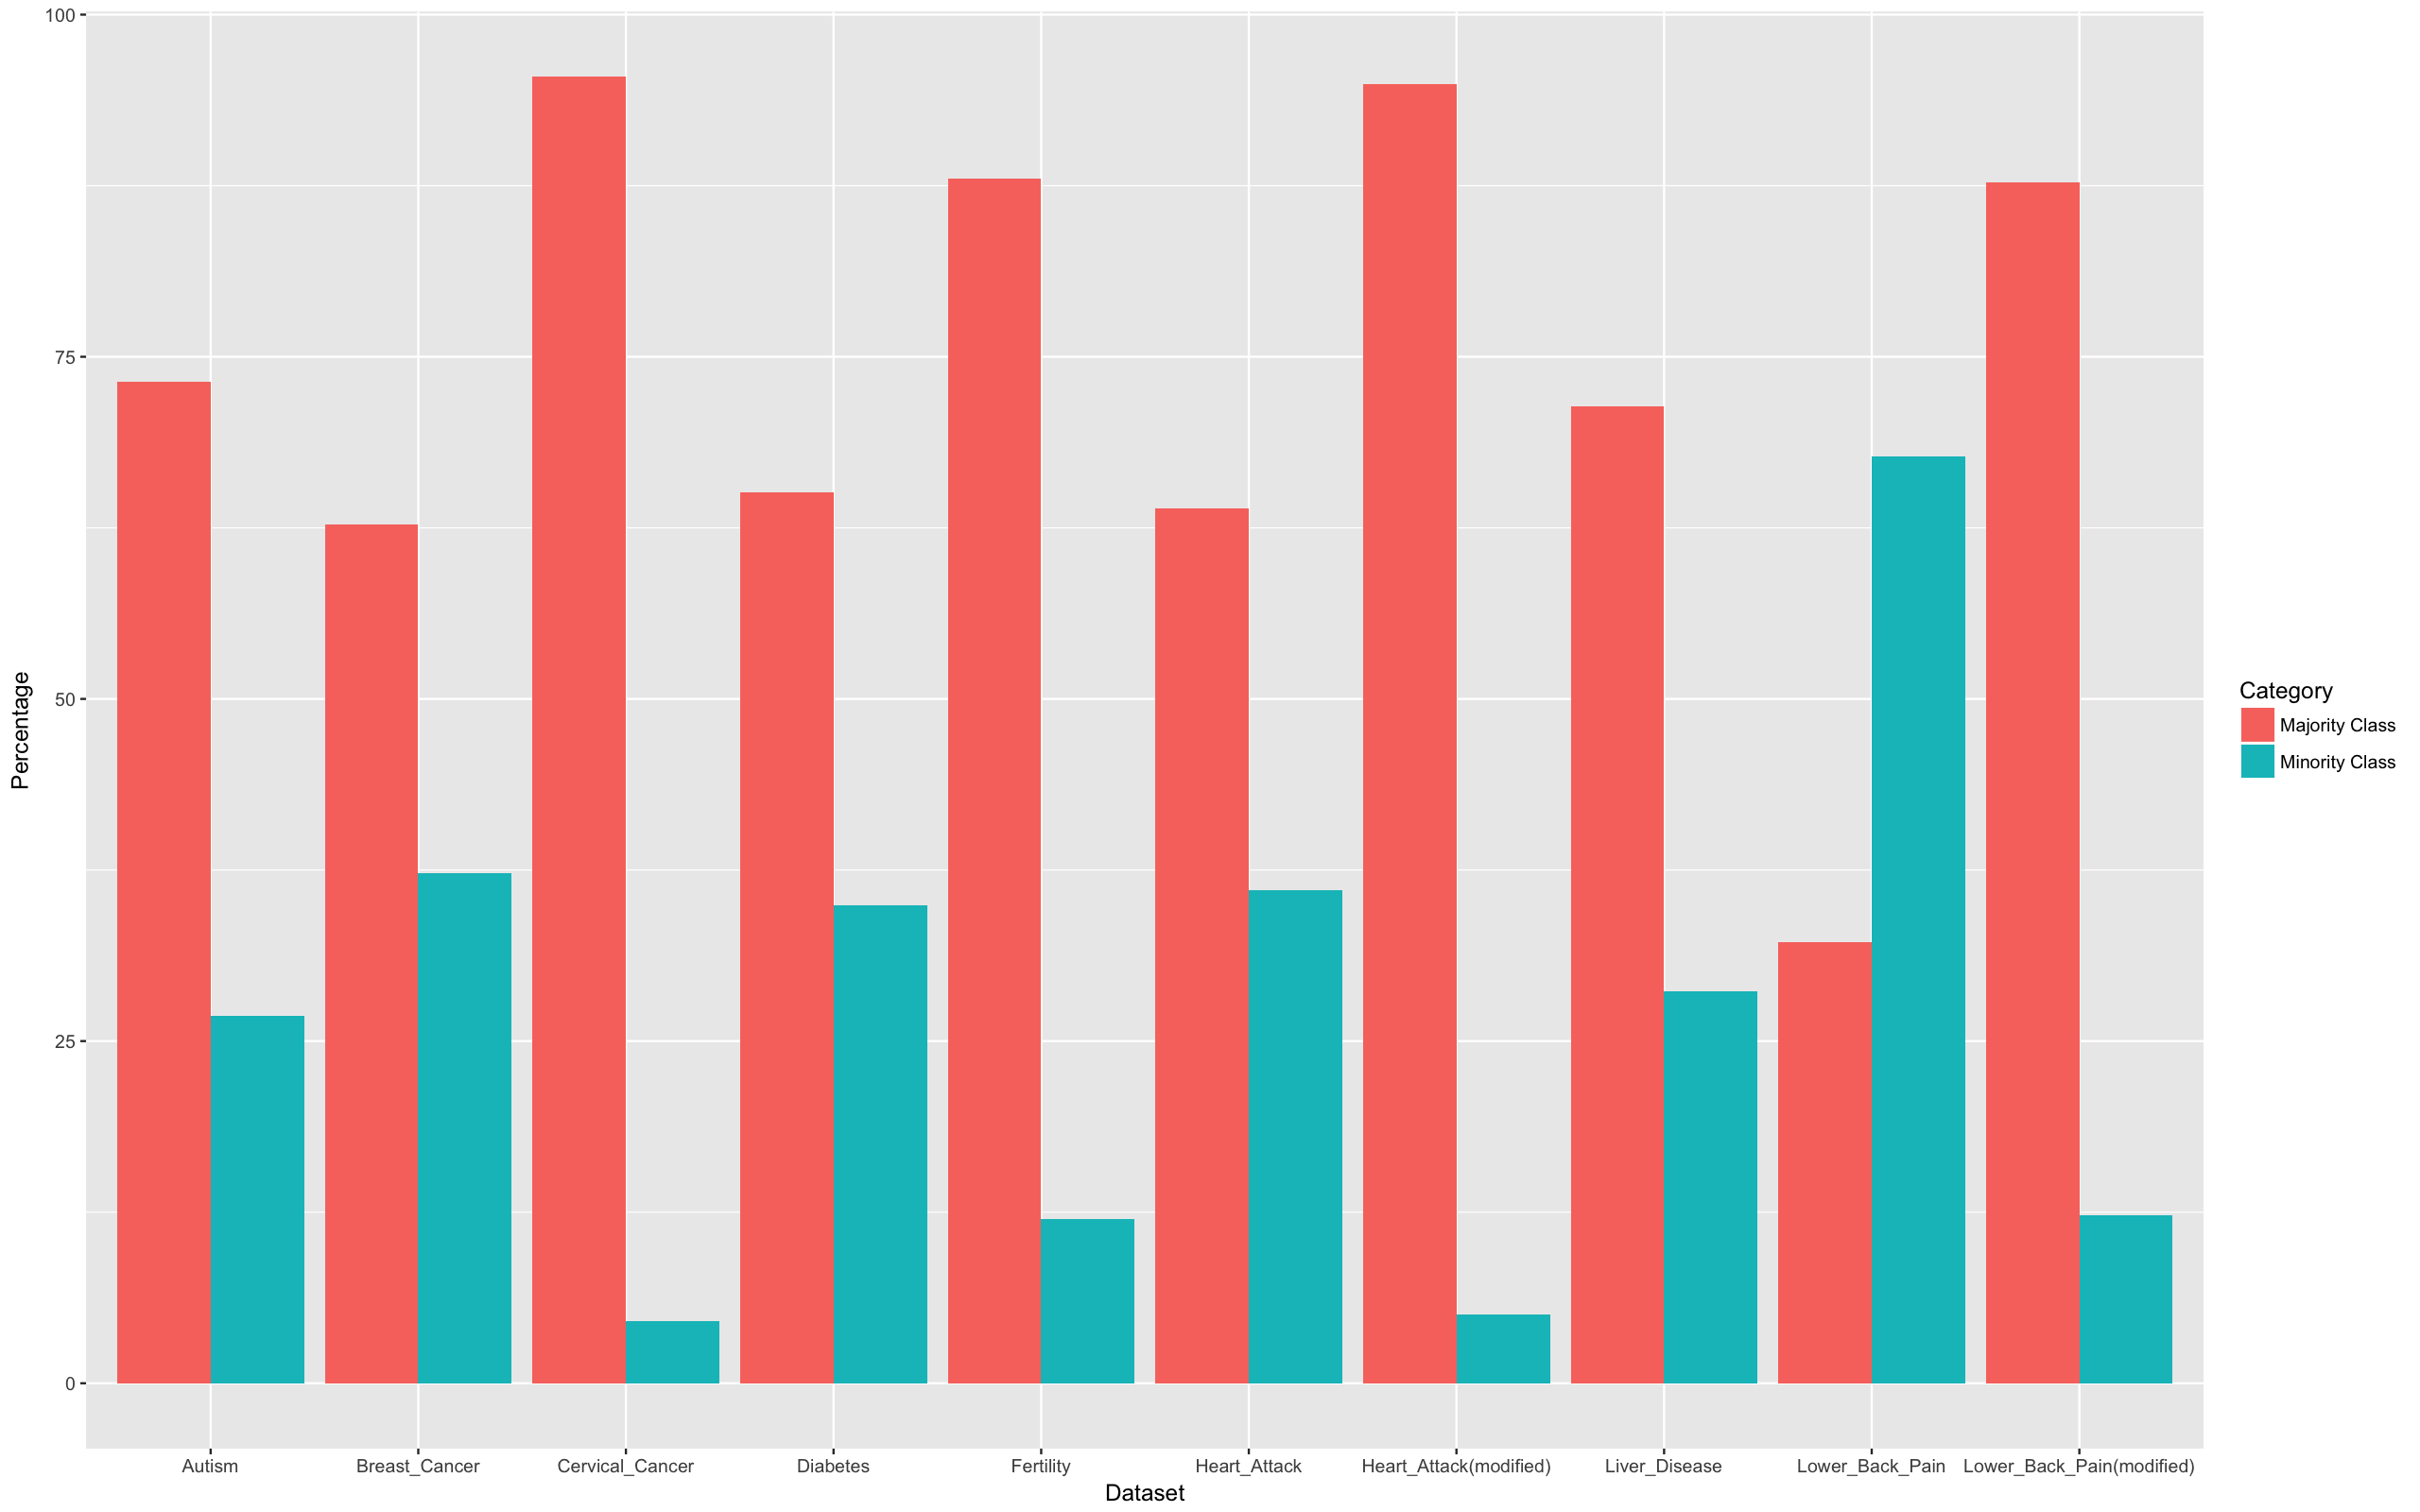
\includegraphics[width=0.95\textwidth]{ThesisTemplate/usingLatex/chapter4Images/figure4_1b.png}
    \caption{Class Distribution of the chosen datasets.\newline In all cases the majority class is the class representing healthy subjects and the minority class is the class representing affected subjects.}
    \label{fig:classDistr}
\end{figure}




\section{Modelling the datasets with Random Forest}
The Random Forest algorithm was used with all the datasets. 
An R script (see linked repository, Experiment1.R and RandomForestModelling.R) was created to classify all 10 datasets and obtain a baseline of the performance that could be obtained on the dataset after pre-processing as detailed in section 4.1.\newline
\subsubsection{Procedure and parameters}
The dataset were uploaded as a list which was iterated through by the R function randomForest(). 
The data split was 70:30 train: test and the number of trees was 128 as Oshiro and colleagues showed that setting the number of trees to higher values mostly only used more CPU but did not improve algorithm performance\citep{MayumiOshiro:ve}. Proximity and importance were both set as true.\newline
The RandomForestModelling.R script output  a data frame containing performance metrics (Accuracy, Precision, Sensitivity and F1 score) of the algorithm for each dataset.\newline
Parameters pertaining to the randomForest() function were modifiable through the randomForestModelling function created in the script so that different situations could be easily modelled.\newline


\section{Modelling the datasets with data-level solutions applied}
\subsection{Under-sampling of the majority class}
An R script was created to fit Random Forest to the datasets after under sampling the majority class in an attempt to address the class imbalance.\newline
Under-sampling means that a proportion of the majority class will be discarded at random with a view to create a more balanced dataset(The diagram in figure 4.2 illustrate under-sampling).\newline
Under-sampling leads to loss of data and though it is expected some metrics will improve, it is also likely that others will worsen; for example precision may increase but sensitivity may decrease.\newline

\begin{figure}[!htbp]
    \centering
    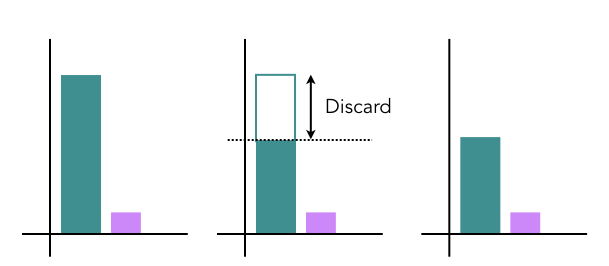
\includegraphics[width=0.9\textwidth]{ThesisTemplate/usingLatex/chapter4Images/Figure2001.png}
    \caption{Under-sampling the majority class. A proportion of the data in the majority class is discarded resulting in more balanced dataset}
    \label{fig:UnderSampling}
\end{figure}


A function to retain different proportion of each class to include in the experiment was devised. Several different percentages of majority class data were tested, while always retained 100 \% of the minority class.\newline
The proportion of each class to include for input in the Random Forest algorithm can be changed as parameters of the function.\newline
The default value for the function was 40\% of the majority class and 100\% of the minority class retained.\newline
Three different values were tested for under-sampling of the majority class:
\begin{itemize}
    \item 40\% of majority class retained
    \item 60\% of majority class retained
    \item 75\% of majority class retained
\end{itemize}

In all cases 100\% of the minority class was retained.\newline
The modified datasets were then fed through the RandomForestModelling script and the accuracy, sensitivity precision and F1 score were recorded to evaluate the effects of the under-sampling on the performance of the algorithm for each dataset.\newline



\subsection{Oversampling of the minority class}
In order to address the class imbalance, this experiment examined the effect of oversampling the minority class. To achieve oversampling, the Synthetic Minority Oversampling Technique or SMOTE \citep{Chawla:2002ty} was applied. \newline 
This technique creates new data points for the minority class from existing data by considering a number of the closest neigbouring points to each existing data points.Figure 4.3 illustrates the over-sampling of minority class by SMOTE. The DMwR package in R contains the smote() function which implements the SMOTE algorithm in R \citep{Anonymous:bPzTqa7x}.\newline

\begin{figure}[!htbp]
    \centering
    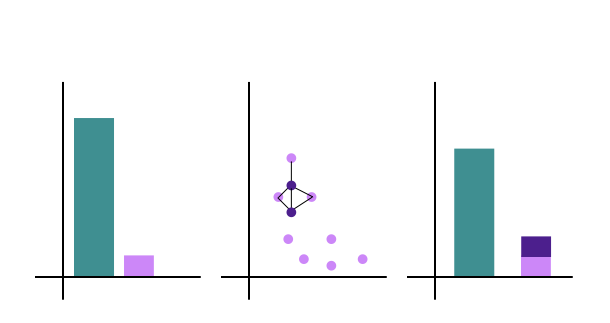
\includegraphics[width=0.9\textwidth]{ThesisTemplate/usingLatex/chapter4Images/Figure2002.png}
    \caption{Over-sampling the minority class. New data points for the minority class are created from existing cases, resulting in a more balanced dataset}
    \label{fig:OverSample}
\end{figure}


The number of existing neighbouring data points to be considered is the \textbf{parameter k} of the smote() function and can be set experimentally to give best results.\newline
The \textbf{k value} is set by default at k=5. However, if k exceeds the number of minority class observations in the training set, an error will occur as there will not be enough points to create the new data point.\newline
Two other parameters need to be set for the function: 
\begin{itemize}
    \item \textbf{perc.over}to set the number of extra cases from the minority class are generated. This is typically a value above 100 so that for each case of the minority class in the original dataset, perc.over/100 new cases will be created.
    \item \textbf{perc.under} controls the number of proportion of cases of the majority class that will be randomly selected for the final balanced dataset. This is calculated based on the the number of newly created minority class cases. 
\end{itemize}

The smote() function is applied only to the training set, in order to train the model,  not the testing set.\newline
The k value used when applying smote to the non modified datasets was k=4. If k was set to a value higher than 4, if the case of those datasets that contained few observations in the minority class after splitting into train and test set, an error was obtained. This was set experimentally but was found to generate good results for the datasets used in this project.\newline
The parameters per.under and perc.over were set at 100 and 200, respectively (so that the new class distribution would be 1:1 majority:minority classes) for the following datasets: Autism, Breast Cancer, Cervical Cancer, Diabetes, Fertility, Low back Pain, Heart Attack and Liver.
The smote() function was applied to the Fertillity, Modified Heart Attack dataset and Low Back Pain dataset with separate parameters from the other datasets, as the generally lower number of observation existing in the sample meant that too few majority class observations were retained. The parameters for these datasets were 200, 600 and k= 4.

\begin{table}[ht]
\centering
\begin{tabular}{lrrr}
  \hline
  \rowcolor{LightCyan}
Dataset & k value & perc.over & perc.under \\ 
  \hline
  AuSDf & 4 & 200 & 100  \\ 
  BCDf & 4 &  200 & 100 \\ 
  CCDf & 4 &  200 & 100\\ 
  DiabetesDf & 4 & 200 & 100 \\ 
  FertDf & 4 &  600 & 200 \\ 
  HAPDf & 4&  200 & 100 \\ 
  LBPDf & 4 &  200 & 100 \\ 
  LiverDf & 4 &  200 & 100 \\
  modHA & 4 & 800 & 200 \\
  modLBP & 4 & 800 & 200 \\
   \hline
\end{tabular}
\label{tab:smoteParam}
\end{table}




\section{Conclusions}
Three different sets of experiments were carried on all eight datasets with a view to compare the resulting accuracy, precision, sensitivity and F1 score for each dataset in each situation. The results will be plotted and discussed in chapter 5.



\chapter{Evaluation \& Testing}\label{ch:Evaluation}

\section{Exploratory Data Analysis}
\subsection{Data Overview}
Description of each dataset (refer to graphs as appendices)- Replacement of n/a value to mean values

\subsection{Class distribution}


\begin{table}[ht]
\centering
\begin{tabular}{lrl}
  \hline
Dataset & Percentage & Category \\ 
  \hline
Cervical\_Cancer & 95.45 & Majority Class \\ 
  Cervical\_Cancer & 4.55 & Minority Class \\ 
  Breast\_Cancer & 62.74 & Majority Class \\ 
  Breast\_Cancer & 37.26 & Minority Class \\ 
  Liver\_Disease & 71.36 & Majority Class \\ 
  Liver\_Disease & 28.64 & Minority Class \\ 
  Diabetes & 65.10 & Majority Class \\ 
  Diabetes & 34.90 & Minority Class \\ 
  Lower\_Back\_Pain & 32.26 & Majority Class \\ 
  Lower\_Back\_Pain & 67.74 & Minority Class \\ 
  Lower\_Back\_Pain(modified) & 87.72 & Majority Class \\ 
  Lower\_Back\_Pain(modified) & 12.28 & Minority Class \\ 
  Heart\_Attack & 63.95 & Majority Class \\ 
  Heart\_Attack & 36.05 & Minority Class \\ 
  Heart\_Attack(modified) & 94.95 & Majority Class \\ 
  Heart\_Attack(modified) & 5.05 & Minority Class \\ 
  Autism & 73.15 & Majority Class \\ 
  Autism & 26.85 & Minority Class \\ 
  Fertility & 88.00 & Majority Class \\ 
  Fertility & 12.00 & Minority Class \\ 
   \hline
\end{tabular}
\end{table}

\begin{figure}[H]
    \centering
    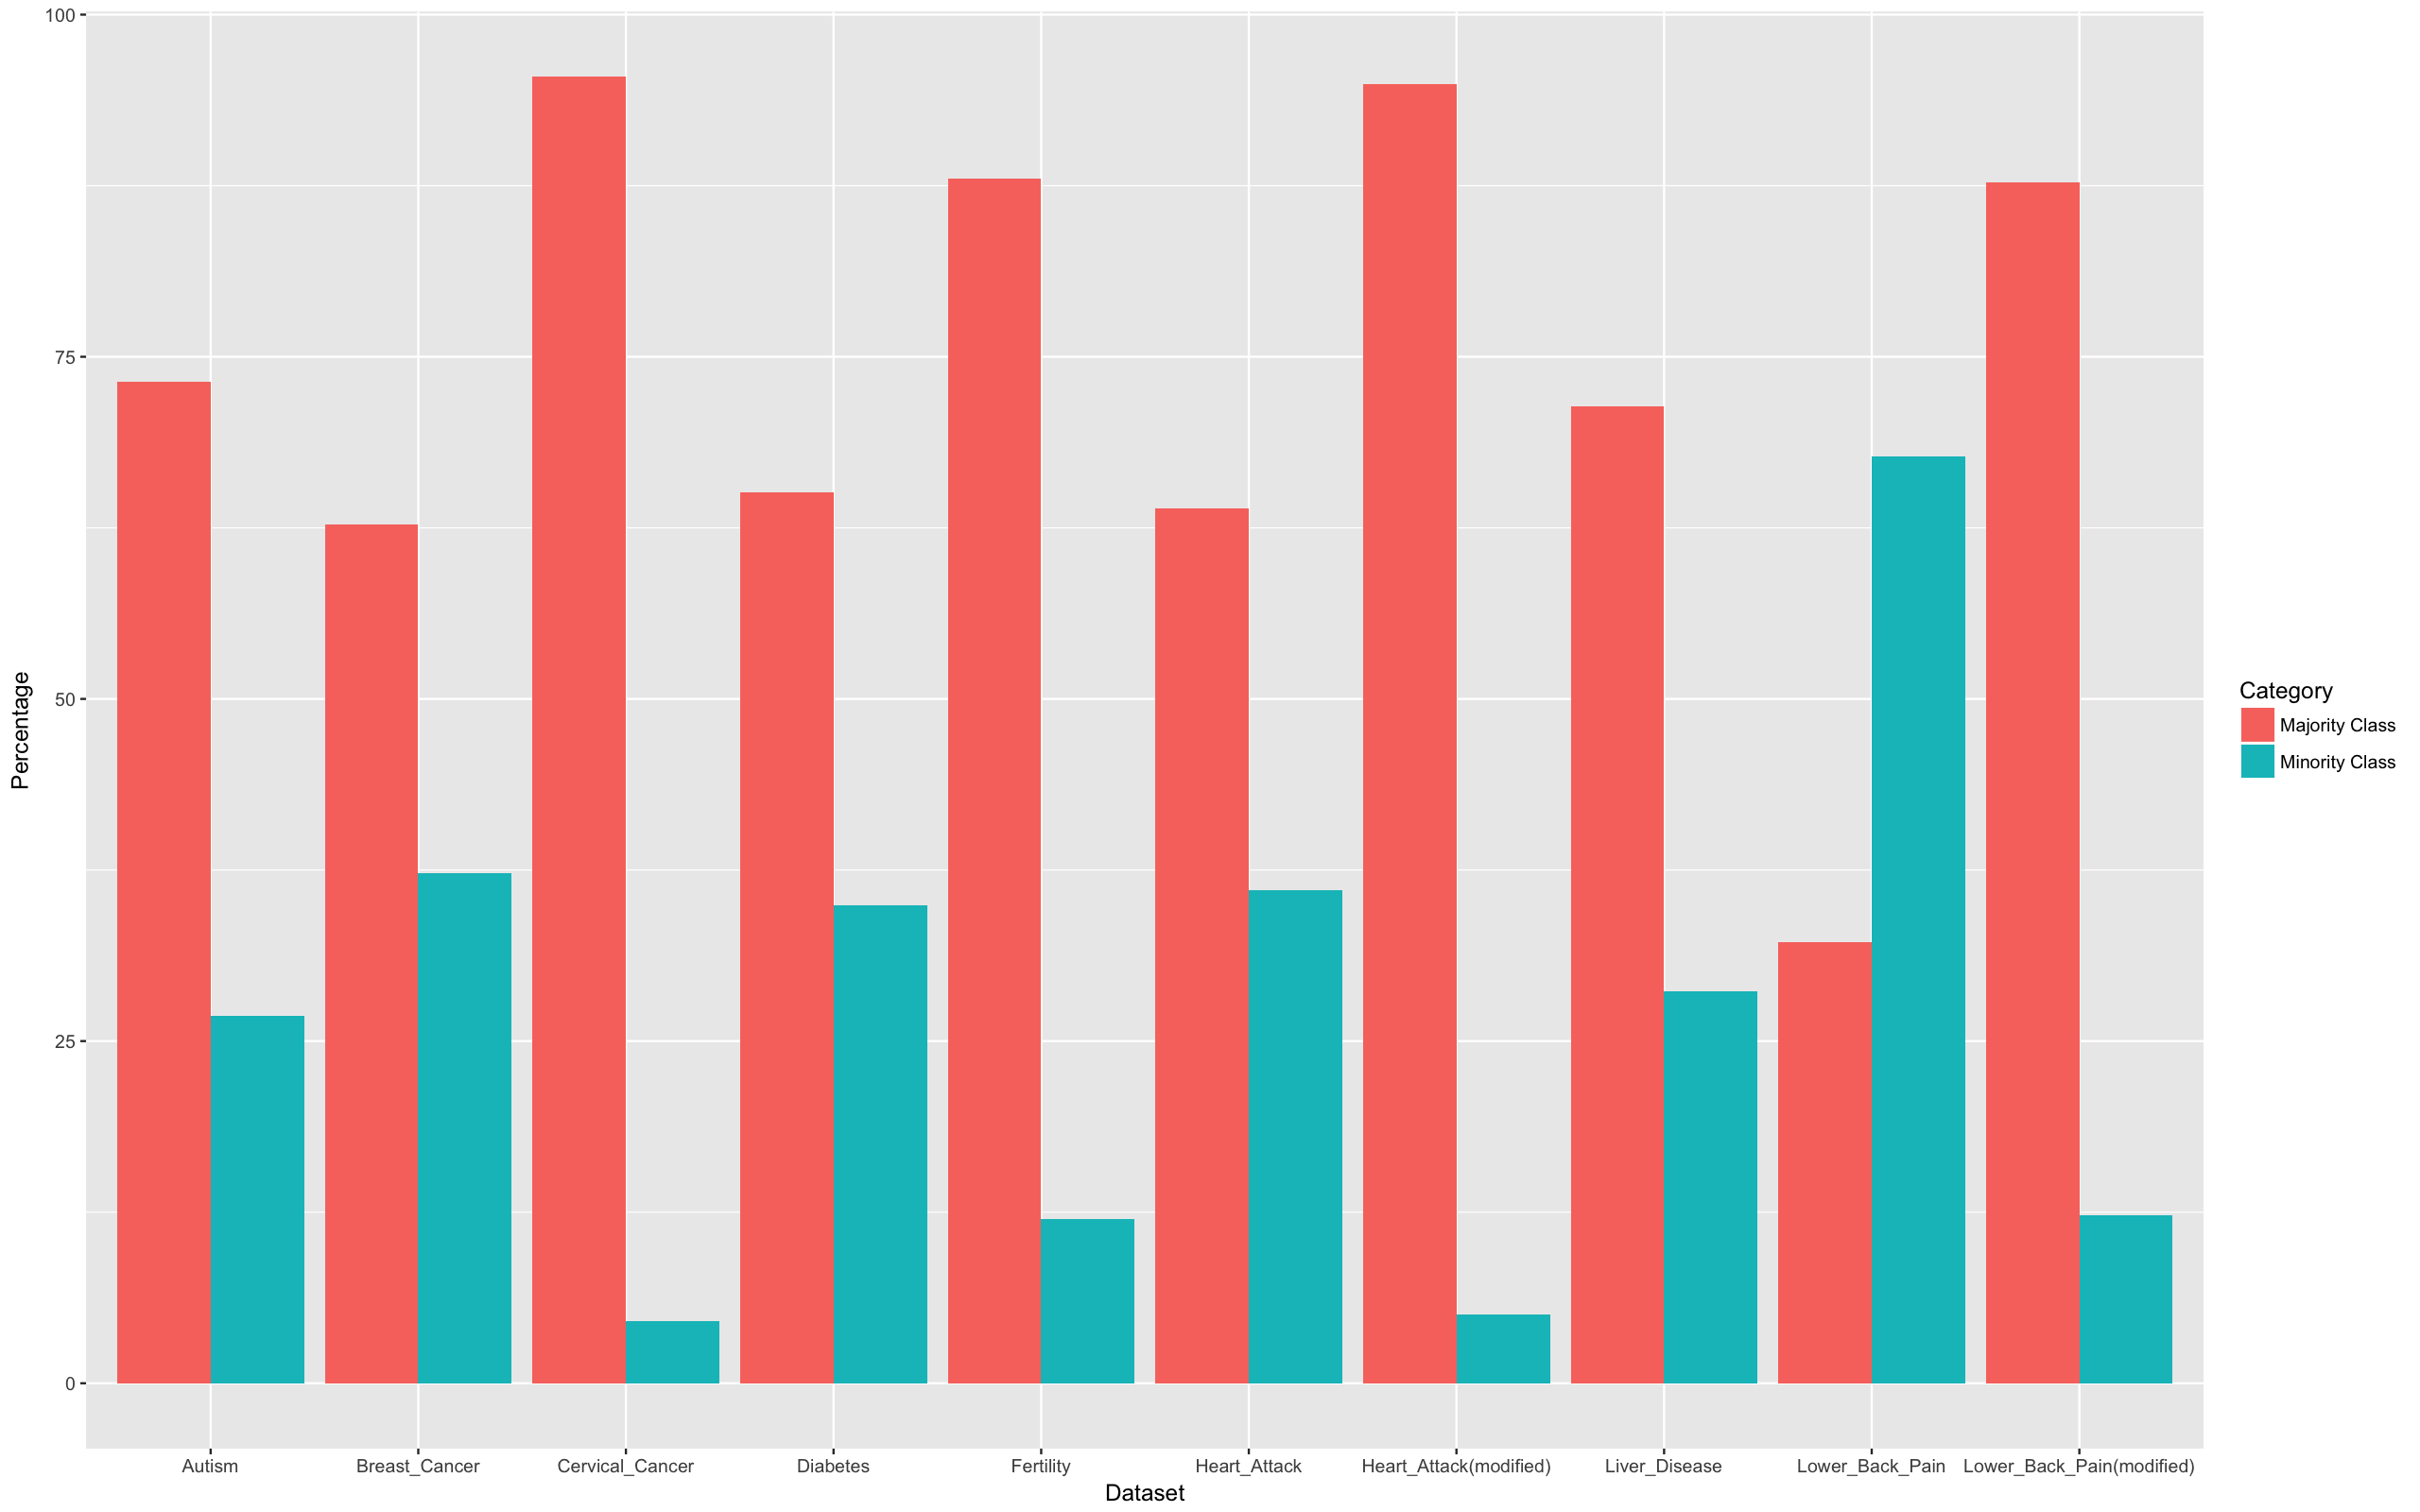
\includegraphics[width=0.8\textwidth]{ThesisTemplate/usingLatex/chapter4Images/figure4_1b.png}
    \caption{Class Distribution of the chosen datasets.\newline In all cases the majority class is the class representing healthy subjects and the minority class is the class representing affected subjects. In the case of the lower back pain dataset, the class representing the "abnormal" patients counts more instances than the the class representing the "normal" patients, however the terms minority and majority were kept for consistency with the other datasets.}
    \label{fig:my_label}
\end{figure}
\section{Modelling the datasets}
\subsection{Random Forest}
\begin{table}[ht]
\centering
\begin{tabular}{lrrrr}
  \hline
Dataset & Accuracy & Sensitivity & Precision & F1Score \\ 
  \hline
AuSDf & 100.00 & 1.00 & 1.00 & 1.00 \\ 
  BCDf & 91.67 & 0.86 & 0.94 & 0.89 \\ 
  CCDf & 93.75 & 0.33 & 0.45 & 0.38 \\ 
  DiabetesDf & 74.12 & 0.56 & 0.72 & 0.63 \\ 
  FertDf & 93.10 & 0.00 &  &  \\ 
  HAPDf & 90.80 & 0.83 & 0.89 & 0.86 \\ 
  LBPDf & 81.52 & 0.90 & 0.84 & 0.87 \\ 
  LiverDf & 71.68 & 0.35 & 0.58 & 0.44 \\ 
   \hline
\end{tabular}
\end{table}
\subsection{Support Machine Vector}
\subsection{K-Nearest Neighbour}
\subsection{Naive  Bayes}
\section{Modelling the datasets with data-level solutions applied}
\subsection{Undersampling of the majority class}
undersampling majority class 40\%
\begin{table}[ht]
\centering
\begin{tabular}{lrrrr}
  \hline
Dataset & Accuracy & Sensitivity & Precision & F1Score \\ 
  \hline
AuSDf & 100.00 & 1.00 & 1.00 & 1.00 \\ 
  BCDf & 94.23 & 0.98 & 0.93 & 0.96 \\ 
  CCDf & 95.45 & 0.75 & 0.82 & 0.78 \\ 
  DiabetesDf & 69.06 & 0.88 & 0.62 & 0.73 \\ 
  FertDf & 92.31 & 0.67 & 1.00 & 0.80 \\ 
  HAPDf & 81.13 & 0.90 & 0.80 & 0.85 \\ 
  LBPDf & 93.06 & 1.00 & 0.92 & 0.96 \\ 
  LiverDf & 70.71 & 0.86 & 0.62 & 0.72 \\ 
   \hline
\end{tabular}
\end{table}

undersampling majority class 60\%
\begin{table}[ht]
\centering
\begin{tabular}{lrrrr}
  \hline
Dataset & Accuracy & Sensitivity & Precision & F1Score \\ 
  \hline
AuSDf & 100.00 & 1.00 & 1.00 & 1.00 \\ 
  BCDf & 96.03 & 0.94 & 0.98 & 0.96 \\ 
  CCDf & 92.50 & 0.61 & 0.69 & 0.65 \\ 
  DiabetesDf & 70.24 & 0.78 & 0.65 & 0.71 \\ 
  FertDf & 77.78 & 0.00 & 0.00 &  \\ 
  HAPDf & 79.69 & 0.69 & 0.92 & 0.79 \\ 
  LBPDf & 78.75 & 0.92 & 0.82 & 0.86 \\ 
  LiverDf & 64.75 & 0.46 & 0.54 & 0.49 \\ 
   \hline
\end{tabular}
\end{table}

undersampling majority class 75\%
\begin{table}[ht]
\centering
\begin{tabular}{lrrrr}
  \hline
Dataset & Accuracy & Sensitivity & Precision & F1Score \\ 
  \hline
AuSDf & 100.00 & 1.00 & 1.00 & 1.00 \\ 
  BCDf & 95.10 & 0.90 & 1.00 & 0.95 \\ 
  CCDf & 95.38 & 0.74 & 0.78 & 0.76 \\ 
  DiabetesDf & 75.26 & 0.64 & 0.70 & 0.67 \\ 
  FertDf & 85.71 & 0.50 & 0.33 & 0.40 \\ 
  HAPDf & 83.33 & 0.75 & 0.81 & 0.78 \\ 
  LBPDf & 86.90 & 0.94 & 0.90 & 0.92 \\ 
  LiverDf & 61.70 & 0.31 & 0.52 & 0.39 \\ 
   \hline
\end{tabular}
\end{table}


\subsection{Oversampling of the minority class}
Oversampling using SMOTE (retain majority class, oversample 100\%)
100, 400
table showing training set distribution before and after smote
\begin{table}[ht]
\centering
\begin{tabular}{lrrrr}
  \hline
Dataset & MajorityClass & MinorityClass & NewMajorityClass & NewMinorityClass \\ 
  \hline
AuSDf & 353 & 140 & 560 & 280 \\ 
  BCDf & 258 & 143 & 572 & 286 \\ 
  CCDf & 573 &  29 & 116 &  58 \\ 
  DiabetesDf & 362 & 178 & 712 & 356 \\ 
  FertDf &  61 &  10 &  40 &  20 \\ 
  HAPDf & 131 &  76 & 304 & 152 \\ 
  LBPDf &  71 & 147 & 142 & 284 \\ 
  LiverDf & 297 & 113 & 452 & 226 \\ 
  subHAPDf & 134 &   7 &  28 &  14 \\ 
  subLBPDf &  74 &   8 &  32 &  16 \\ 
   \hline
\end{tabular}
\end{table}


\begin{table}[ht]
\centering
\begin{tabular}{lrrrr}
  \hline
Dataset & Accuracy & Sensitivity & Precision & F1Score \\ 
  \hline
AuSDf & 100.00 & 1.00 & 1.00 & 1.00 \\ 
  BCDf & 93.45 & 0.90 & 0.94 & 0.92 \\ 
  CCDf & 97.66 & 0.90 & 0.64 & 0.75 \\ 
  DiabetesDf & 75.00 & 0.62 & 0.71 & 0.66 \\ 
  FertDf & 75.86 & 0.50 & 0.14 & 0.22 \\ 
  HAPDf & 88.51 & 0.83 & 0.83 & 0.83 \\ 
  LBPDf & 78.26 & 0.84 & 0.84 & 0.84 \\ 
  LiverDf & 71.10 & 0.56 & 0.54 & 0.55 \\ 
  subHAPDf & 92.98 & 0.33 & 0.33 & 0.33 \\ 
  subLBPDf & 93.75 & 0.67 & 1.00 & 0.80 \\ 
   \hline
\end{tabular}
\end{table}


Repeat experiment to exclude modified heart attack and lowback pain dataset and do smote on those separately
\begin{table}[ht]
\centering
\begin{tabular}{lrrrr}
  \hline
Dataset & MajorityClass & MinorityClass & NewMajorityClass & NewMinorityClass \\ 
  \hline
AuSDf & 353 & 140 & 560 & 280 \\ 
  BCDf & 258 & 143 & 572 & 286 \\ 
  CCDf & 573 &  29 & 116 &  58 \\ 
  DiabetesDf & 362 & 178 & 712 & 356 \\ 
  FertDf &  61 &  10 &  40 &  20 \\ 
  HAPDf & 131 &  76 & 304 & 152 \\ 
  LBPDf &  71 & 147 & 142 & 284 \\ 
  LiverDf & 297 & 113 & 452 & 226 \\ 
   \hline
\end{tabular}
\end{table}

\begin{table}[ht]
\centering
\begin{tabular}{lrrrr}
  \hline
Dataset & Accuracy & Sensitivity & Precision & F1Score \\ 
  \hline
AuSDf & 100.00 & 1.00 & 1.00 & 1.00 \\ 
  BCDf & 93.45 & 0.90 & 0.94 & 0.92 \\ 
  CCDf & 97.66 & 0.90 & 0.64 & 0.75 \\ 
  DiabetesDf & 75.00 & 0.62 & 0.71 & 0.66 \\ 
  FertDf & 75.86 & 0.50 & 0.14 & 0.22 \\ 
  HAPDf & 88.51 & 0.83 & 0.83 & 0.83 \\ 
  LBPDf & 78.26 & 0.84 & 0.84 & 0.84 \\ 
  LiverDf & 71.10 & 0.56 & 0.54 & 0.55 \\ 
   \hline
\end{tabular}
\end{table}

Now do RF on HA and LBP
\begin{table}[ht]
\centering
\begin{tabular}{lrrrr}
  \hline
Dataset & MajorityClass & MinorityClass & NewMajorityClass & NewMinorityClass \\ 
  \hline
subHAPDf & 134 &   7 &  84 &  21 \\ 
  subLBPDf &  74 &   8 &  96 &  24 \\ 
   \hline
\end{tabular}
\end{table}

\begin{table}[ht]
\centering
\begin{tabular}{lrrrr}
  \hline
Dataset & Accuracy & Sensitivity & Precision & F1Score \\ 
  \hline
subHAPDf & 92.98 & 0.33 & 0.33 & 0.33 \\ 
  subLBPDf & 87.50 & 0.33 & 1.00 & 0.50 \\ 
   \hline
\end{tabular}
\end{table}

do fertility on its own
\begin{table}[ht]
\centering
\begin{tabular}{lrrrr}
  \hline
Dataset & MajorityClass & MinorityClass & NewMajorityClass & NewMinorityClass \\ 
  \hline
FertDf &  61 &  10 & 120 &  30 \\ 
   \hline
\end{tabular}
\end{table}

\begin{table}[ht]
\centering
\begin{tabular}{lrrrr}
  \hline
Dataset & Accuracy & Sensitivity & Precision & F1Score \\ 
  \hline
FertDf & 96.55 & 0.50 &   1 & 0.67 \\ 
   \hline
\end{tabular}
\end{table}


\subsection{k-mean}

\section{Conclusions}

The main conclusions for this chapter.



\chapter{Conclusion}\label{ch:Conclusion}
This project has investigated potential data-level solutions that can be implemented to reduce the negative impact of imbalanced datasets on the performance of algorithms in machine learning, particularly in the context of healthcare and medical diagnostics.\newline
The approach was to first determine the baseline performance of Random Forest on 8 datasets (plus modified versions of two of the chosen sets with greater class imbalance). Second, under-sampling of the data was carried out in various proportions and the performance metrics measured again. In a third experiment, over-sampling by SMOTE was carried out and the performance metrics measured. Accuracy, Precision, Sensitivity and F1 score were recorded in all cases and compared between experiments.
The outcomes of each experiment were detailed in chapter 5 and the work carried out in this project shows that no single solution improved the performance of Random Forest for all datasets.\newline
Performance must first be clearly defined and with medical diagnostic in mind, it was decided that sensitivity would be considered a more important parameter than precision. Overall accuracy was still considered important though small decreases in accuracy could be tolerated if sensitivity was significantly increased. The F1 score is a more ambiguous measure to consider as it is the harmonic mean of both precision and sensitivity. An increase in the F1 score is beneficial though it is unclear if it is due to a large increase in sensitivity and a constant or slightly reduced precision, or the opposite, or both measure increasing. It does give an idea of the balance between both measures and a decrease in F1 score largely points to a decrease in algorithm performance.\newline

\section{Conclusions}
The results to the experiments carried out showed that for a given dataset under-sampling was a better data-level solution to apply to improve the performance of Random Forest, as has been suggested by others \citep{Rekha:2019uu}, though the opposite has also been found. Working with the same Cervical Cancer dataset and a Decision Tree algorithm, Al-Wesabi and colleagues \citep{AlWesabi:hx} found that oversampling was far superior to under-sampling in improving algorithm performance. The parameters for SMOTE used here specifically for the Cervical Cancer dataset lead to a large reduction of data even though the data then contain the same number of positive and negative cases. This may explain the discrepancy between the results of this projects and those reported by Al-Wesabi and colleagues.\newline
The extent to which under-sampling improved the performance of an Random Forest was not constant, although it almost consistently improved sensitivity. In contrast, the effect of SMOTE was more constant across the datasets but less pronounced.\newline
The results obtained with the Fertility dataset and the modified Heart Attack and modified Low Back Pain suggest that another type of algorithm, such a SVM or k-NN may have performed better. The baseline experiment failed to correctly identify any positive cases for the Fertility dataset and this may have been because Random Forest was not best suited to this data environment. This theory could be examined further (see future work) and inform the current results.\newline


\section{Future Work}
Should more time be spent on this project, it would be interesting to investigate the effects of different parameters for SMOTE on the performance of the algorithm.
An attractive idea is that of devising a hybrid strategy for example under-sampling the majority class after having applied SMOTE to the dataset as reported by Liu and colleagues \citep{Liu:2006ij}. This could further improve the performance of the algorithm compared to what is obtain with either technique.\newline
The original plan for this project, as detailed in chapter 3, outlined the comparison of the performance of several algorithms using the same datasets and both under and over-sampling. This has not been carried out due to lack of time, however this could be informative to assess whether the data-level solutions can improve the performance of several different algorithms when used in the same way, i.e. would SMOTE applied with the same parameters to a given dataset result in performance improvement for both a Decision Tree algorithm and k-NN or SVM.\newline
Another aspect discussed in Chapter 3, but not carried out in this project are algorithm level solutions that can be experimented with in order to improve the performance of an algorithm for a given dataset. This type of solution would most likely be very data-specific, but very suited to an algorithm such as SVM where learning cost can be factored in as parameter.



\footnotesize  %NOTE: reduced the size of the text for the bibliography
%NOTE: set the style for the bibliography and display the references used within the document
\bibliographystyle{agsm}
\bibliography{22_03_19Bib.bib}
\include{bibliography}
\normalsize
\appendix
\chapter{Project Specification}
Summary of the project outline.

\section{Functional Requirements}
some text here

\section{Non-Functional Requirements}
some text here

\chapter{Project Management}
Discussion on how the project was managed. What things impacted the success of the project. How does the continually revised versions of the project plan compare to the initial draft developed at the start of the project. Did everything run according the schedule. Did elements such as exams \& coursework have any impact. 

\chapter{Implementation Appendix}

\begin{figure}[!htbp]
    \centering
    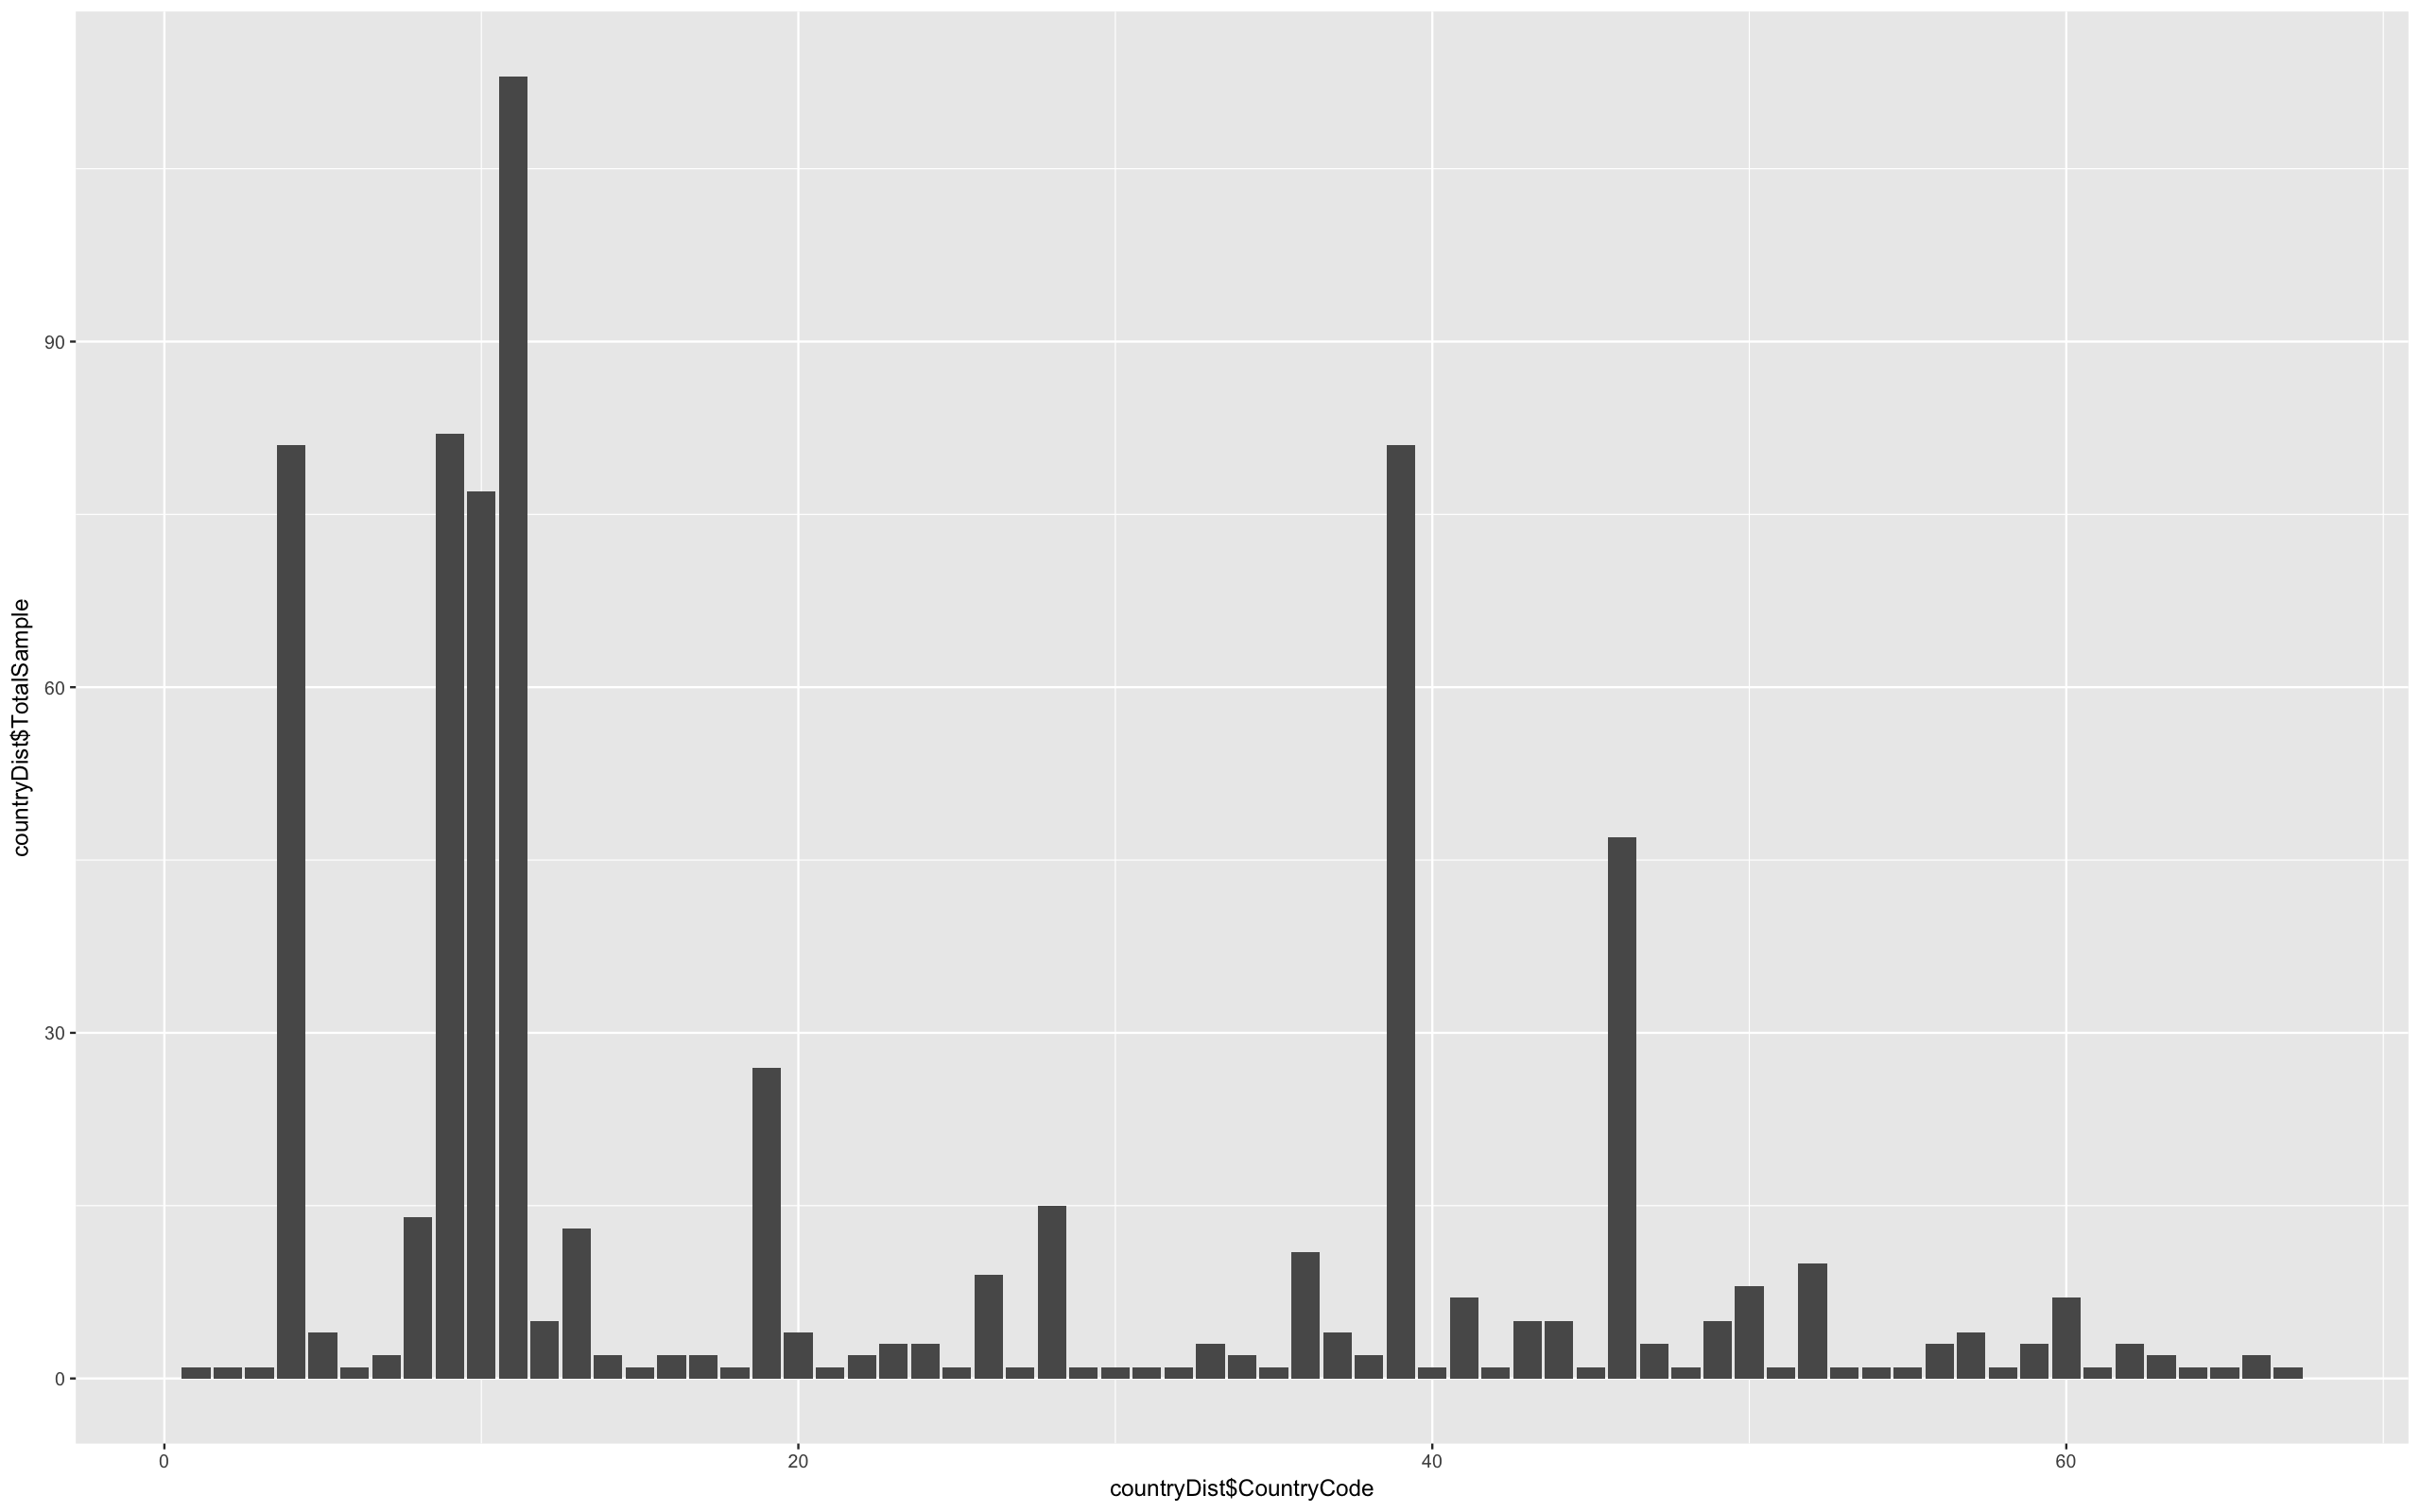
\includegraphics[width=0.9\textwidth]{ThesisTemplate/appendix/images/figure4_2b.png}
    \caption{Distribution of the autism data by country of residence.}
    \label{fig:my_label}
\end{figure}

\chapter{Evaluation Appendix}
\begin{figure}[!htbp]
    \centering
    \begin{minipage}{0.45\textwidth}
        \centering
        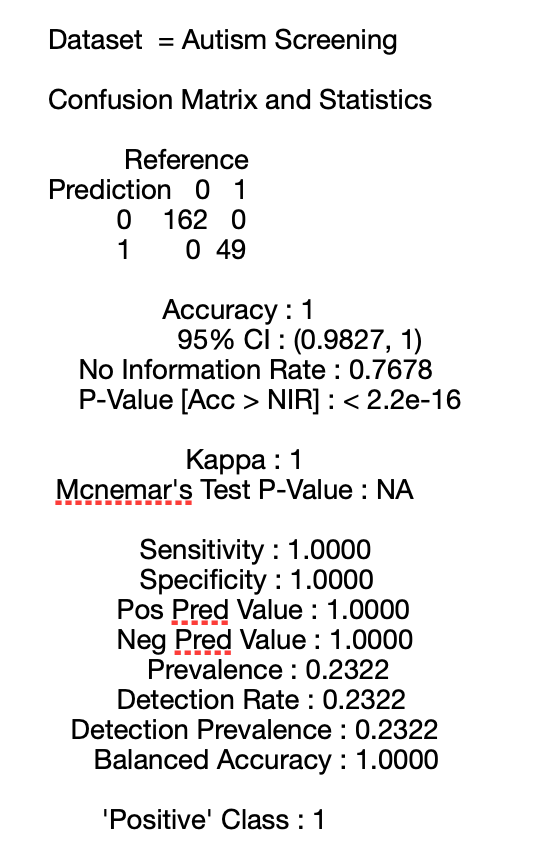
\includegraphics[width=0.9\textwidth]{ThesisTemplate/appendix/images/Chapter5Appendix/Autism.png} 
        \caption{Confusion Matrix output for Random Forest fitted to the Autism Dataset}
        \label{fig:my_label}
    \end{minipage}\hfill
    \begin{minipage}{0.45\textwidth}
        \centering
        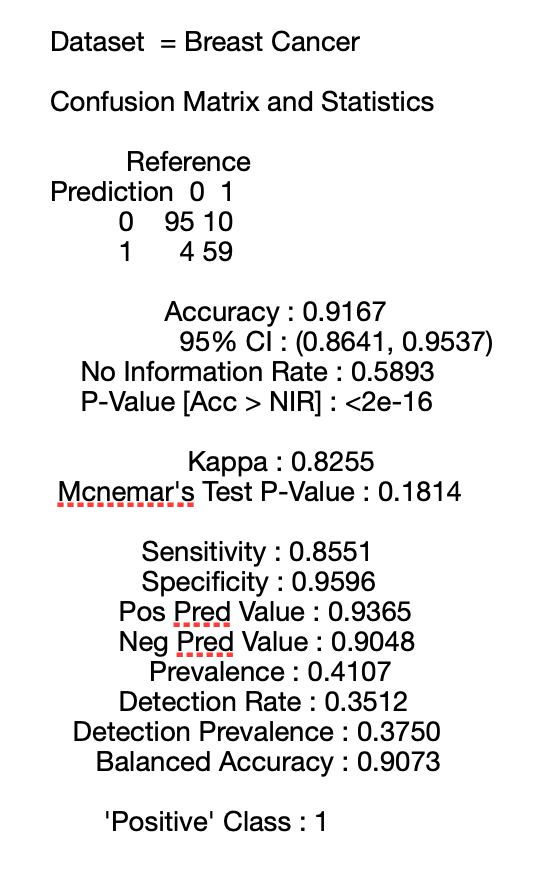
\includegraphics[width=0.9\textwidth]{ThesisTemplate/appendix/images/Chapter5Appendix/BreastCancer.png} 
        \caption{Confusion Matrix output for Random Forest fitted to the Breast Cancer Dataset}
        \label{fig:my_label}
    \end{minipage}
\end{figure}

\begin{figure}[!htbp]
    \centering
    \begin{minipage}{0.45\textwidth}
        \centering
        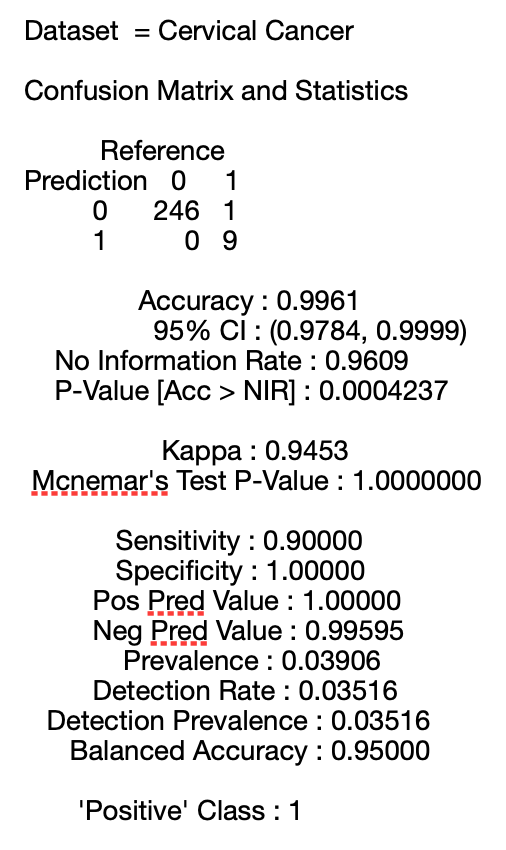
\includegraphics[width=0.9\textwidth]{ThesisTemplate/appendix/images/Chapter5Appendix/CervicalCancer.png} 
        \caption{Confusion Matrix output for Random Forest fitted to the Autism Dataset}
        \label{fig:my_label}
    \end{minipage}\hfill
    \begin{minipage}{0.45\textwidth}
        \centering
        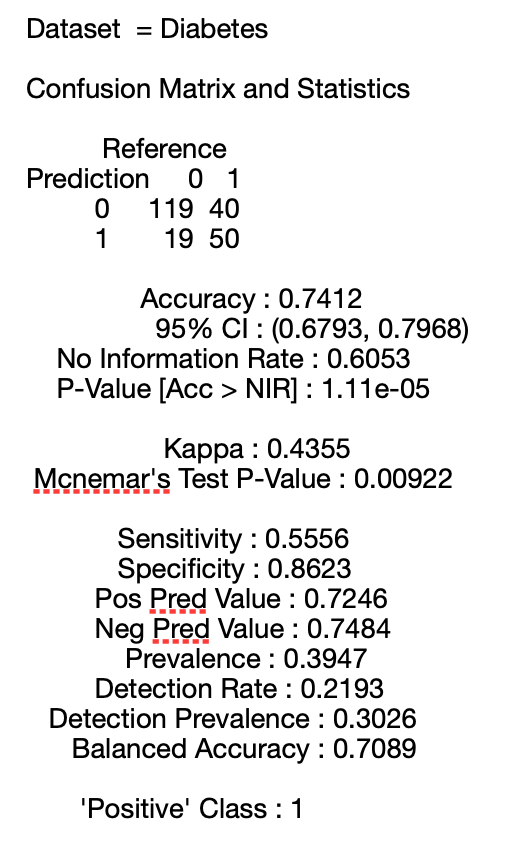
\includegraphics[width=0.9\textwidth]{ThesisTemplate/appendix/images/Chapter5Appendix/Diabetes.png} 
        \caption{Confusion Matrix output for Random Forest fitted to the Breast Cancer Dataset}
        \label{fig:my_label}
    \end{minipage}
\end{figure}

\begin{figure}[!htbp]
    \centering
    \begin{minipage}{0.45\textwidth}
        \centering
        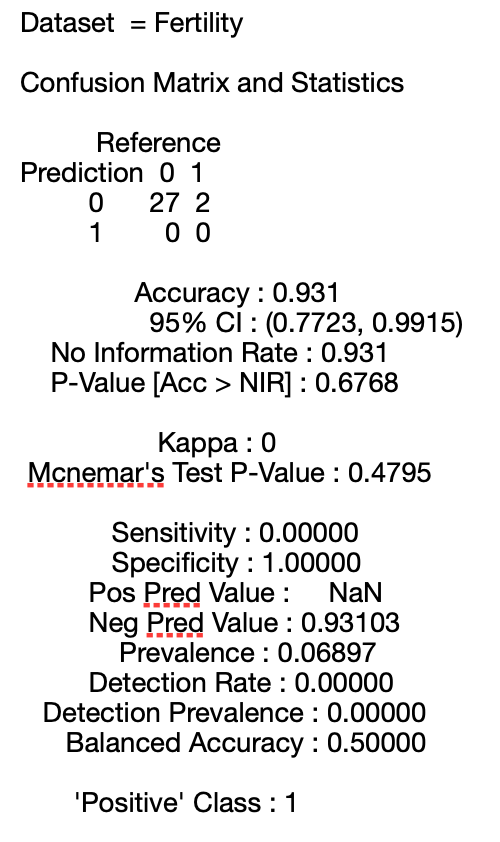
\includegraphics[width=0.9\textwidth]{ThesisTemplate/appendix/images/Chapter5Appendix/Fertility.png} 
        \caption{Confusion Matrix output for Random Forest fitted to the Autism Dataset}
        \label{fig:my_label}
    \end{minipage}\hfill
    \begin{minipage}{0.45\textwidth}
        \centering
        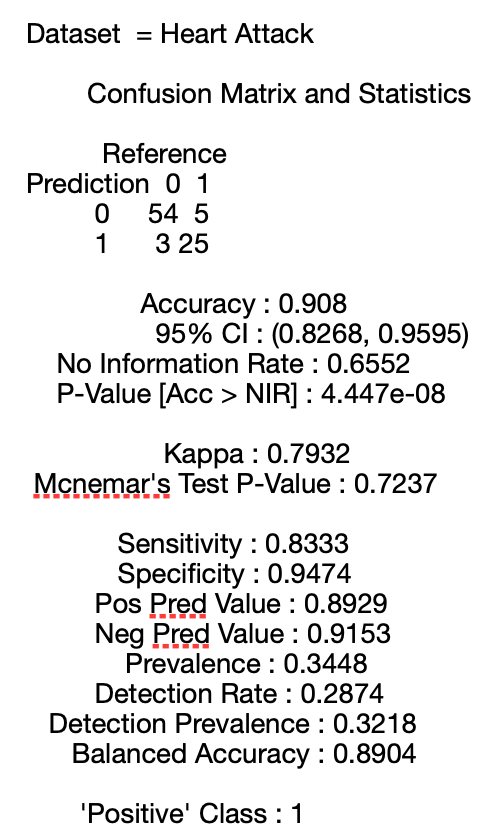
\includegraphics[width=0.9\textwidth]{ThesisTemplate/appendix/images/Chapter5Appendix/HeartAttack.png} 
        \caption{Confusion Matrix output for Random Forest fitted to the Breast Cancer Dataset}
        \label{fig:my_label}
    \end{minipage}
\end{figure}


\begin{figure}[!htbp]
    \centering
    \begin{minipage}{0.45\textwidth}
        \centering
        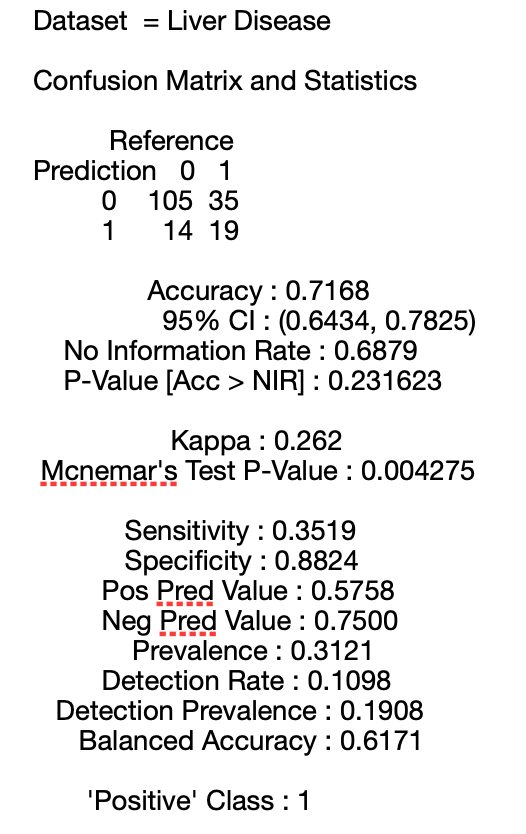
\includegraphics[width=0.9\textwidth]{ThesisTemplate/appendix/images/Chapter5Appendix/LiverDisease.png} 
        \caption{Confusion Matrix output for Random Forest fitted to the Autism Dataset}
        \label{fig:my_label}
    \end{minipage}\hfill
    \begin{minipage}{0.45\textwidth}
        \centering
        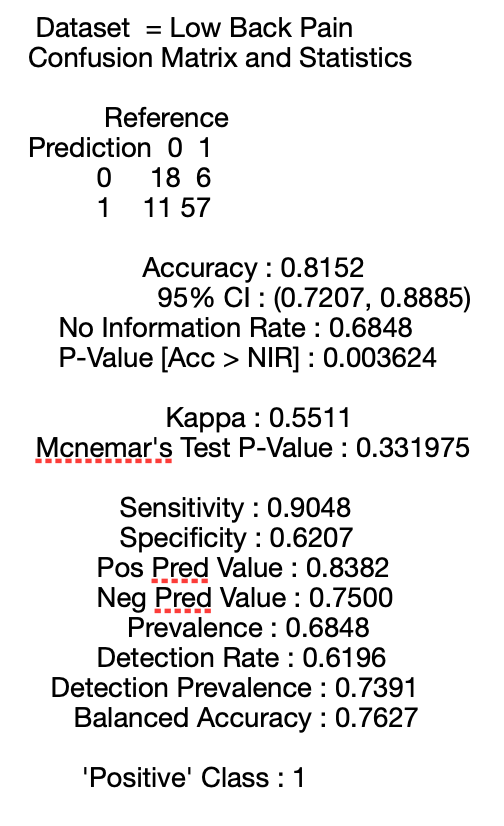
\includegraphics[width=0.9\textwidth]{ThesisTemplate/appendix/images/Chapter5Appendix/LowBackPain.png} 
        \caption{Confusion Matrix output for Random Forest fitted to the Breast Cancer Dataset}
        \label{fig:my_label}
    \end{minipage}
\end{figure}

\begin{figure}[!htbp]
    \centering
    \begin{minipage}{0.45\textwidth}
        \centering
        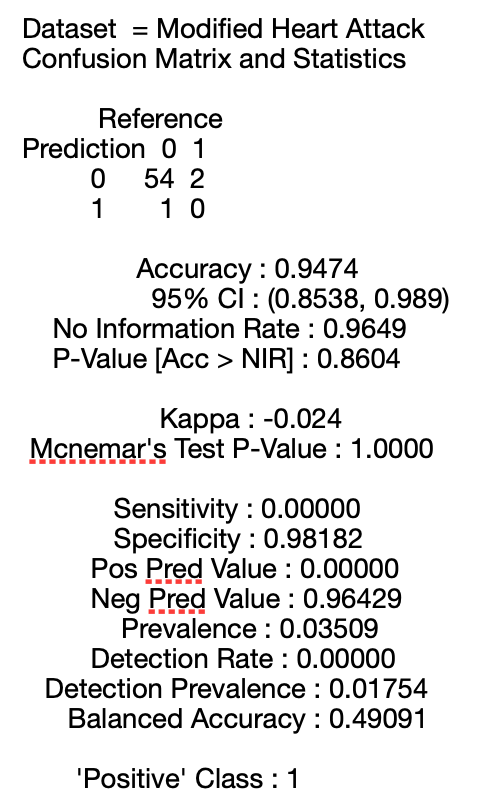
\includegraphics[width=0.9\textwidth]{ThesisTemplate/appendix/images/Chapter5Appendix/modHeartAttack.png} 
        \caption{Confusion Matrix output for Random Forest fitted to the Autism Dataset}
        \label{fig:my_label}
    \end{minipage}\hfill
    \begin{minipage}{0.45\textwidth}
        \centering
        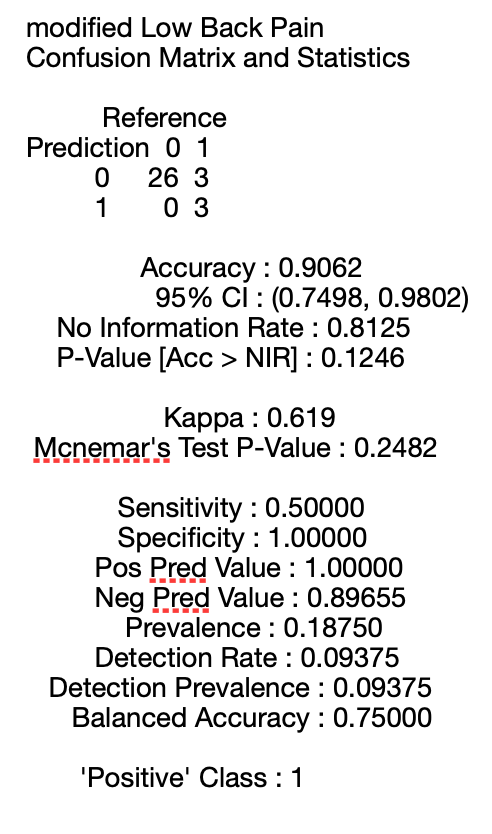
\includegraphics[width=0.9\textwidth]{ThesisTemplate/appendix/images/Chapter5Appendix/modLowBackPain.png} 
        \caption{Confusion Matrix output for Random Forest fitted to the Breast Cancer Dataset}
        \label{fig:my_label}
    \end{minipage}
\end{figure}



 

\chapter{Project Log}








}
\end{document} %NOTE: END of document, nothing after this point
